% =====================================================================
%  A Daily Return-Based Multi-Asset Factor Model
%  Construction, Estimation and Out-of-Sample Validation
%
%  Build:  pdflatex -interaction=nonstopmode factor-model-paper.tex  (twice)
%  or:     python -m scripts.build_paper
% =====================================================================
\documentclass[11pt,a4paper]{article}

\usepackage[T1]{fontenc}
\usepackage[utf8]{inputenc}
\usepackage[english]{babel}
\usepackage{mathpazo}
\usepackage[scaled=0.90]{helvet}
\usepackage{microtype}

\usepackage[a4paper,top=30mm,bottom=28mm,left=32mm,right=32mm]{geometry}
\usepackage{amsmath,amssymb}
\usepackage{booktabs,array,longtable,tabularx}
\usepackage{xcolor}
\usepackage{titlesec}
\usepackage{fancyhdr}
\usepackage[font=small,labelfont=bf,labelsep=period]{caption}
\usepackage{enumitem}
\usepackage{listings}
\usepackage{tikz}
\usetikzlibrary{positioning,shapes.geometric,arrows,fit,backgrounds,calc}
\usepackage[round,authoryear]{natbib}
\usepackage[hidelinks]{hyperref}

% ---------------------------------------------------------------------
%  palette — the same navy and paper tones the application uses
% ---------------------------------------------------------------------
\definecolor{navy}{HTML}{23456B}
\definecolor{ink}{HTML}{1A1A1A}
\definecolor{rule}{HTML}{C9C4BA}
\definecolor{paper}{HTML}{F7F5F0}
\definecolor{brick}{HTML}{8C3A2E}
\definecolor{moss}{HTML}{4A6B4A}

\hypersetup{
  colorlinks=true, linkcolor=navy, urlcolor=navy, citecolor=navy,
  pdftitle={A Daily Return-Based Multi-Asset Factor Model},
  pdfauthor={Bastian Offermann},
  pdfsubject={Factor model construction, estimation and validation},
}

% ---------------------------------------------------------------------
%  headings
% ---------------------------------------------------------------------
\titleformat{\section}
  {\normalfont\sffamily\large\bfseries\color{navy}}{\thesection}{0.8em}{}
\titleformat{\subsection}
  {\normalfont\sffamily\normalsize\bfseries\color{ink}}{\thesubsection}{0.7em}{}
\titleformat{\subsubsection}
  {\normalfont\sffamily\small\bfseries\color{ink}}{\thesubsubsection}{0.6em}{}
\titlespacing*{\section}{0pt}{2.2ex plus 1ex minus .2ex}{1.2ex plus .2ex}
\titlespacing*{\subsection}{0pt}{1.8ex plus 1ex minus .2ex}{0.9ex plus .2ex}

\pagestyle{fancy}
\fancyhf{}
\renewcommand{\headrulewidth}{0.3pt}
\renewcommand{\headrule}{\hbox to\headwidth{\color{rule}\leaders\hrule height \headrulewidth\hfill}}
\fancyhead[L]{\footnotesize\sffamily\color{navy}Daily Return-Based Multi-Asset Factor Model}
\fancyhead[R]{\footnotesize\sffamily\color{navy}\thepage}

\setlength{\parskip}{0.6ex}
\setlength{\parindent}{0pt}
\renewcommand{\arraystretch}{1.18}

% ---------------------------------------------------------------------
%  a boxed note, used for design decisions that would otherwise be lost
% ---------------------------------------------------------------------
\newsavebox{\decisionbox}
\newenvironment{decision}[1]
  {\par\vspace{1.7ex}%
   \begin{lrbox}{\decisionbox}\begin{minipage}{\textwidth}%
   {\color{rule}\rule{\textwidth}{0.4pt}}\par\vspace{0.7ex}
   {\small\sffamily\bfseries\color{navy}#1}\par\vspace{0.35ex}
   \small\itshape}
  {\par\vspace{0.7ex}\noindent{\color{rule}\rule{\textwidth}{0.4pt}}%
   \end{minipage}\end{lrbox}%
   \noindent\usebox{\decisionbox}\par\vspace{1.7ex}}

\lstset{
  basicstyle=\ttfamily\footnotesize,
  keywordstyle=\color{navy}\bfseries,
  commentstyle=\color{moss}\itshape,
  stringstyle=\color{brick},
  backgroundcolor=\color{paper},
  frame=single, rulecolor=\color{rule}, framesep=6pt,
  xleftmargin=2pt, xrightmargin=2pt,
  breaklines=true, showstringspaces=false,
  columns=fullflexible, aboveskip=1.4ex, belowskip=1.4ex,
}

\newcommand{\code}[1]{\texttt{\small #1}}

% =====================================================================
\begin{document}

% ------------------------------- title -------------------------------
\begin{titlepage}
\thispagestyle{empty}
\vspace*{1.4cm}
{\raggedright
{\color{rule}\rule{\textwidth}{0.8pt}}\\[2.2ex]
{\sffamily\LARGE\bfseries\color{navy} A Daily Return-Based\\[0.5ex]
 Multi-Asset Factor Model\par}
\vspace{1.6ex}
{\sffamily\large\color{ink} Construction, Estimation and Out-of-Sample Validation\par}
\vspace{2.0ex}
{\color{rule}\rule{\textwidth}{0.8pt}}\\[3.0ex]
{\large Bastian Offermann\par}
\vspace{0.6ex}
{\small\color{ink} September 2026\par}
}

\vspace{1.6cm}

\begin{minipage}{\textwidth}
\small
\textbf{\sffamily\color{navy}Abstract.}
This paper documents a factor model that estimates exposures from observed returns
alone, without holdings data or look-through. Forty daily factors are constructed
across nine blocks --- equity market, equity style, rates, credit, foreign exchange,
commodities, volatility, liquidity and stress, and alternative risk premia --- from
203 instruments and 53 level series, giving 200{,}072 factor observations from
December 2003 to September 2026. Every model input is a return, and stationarity is
tested rather than assumed: a six-test battery gates the panel, with the
Dickey-Fuller and KPSS tests read jointly because neither alone identifies the
failure that matters. The factor panel is maintained in two forms, raw and
block-orthogonalised, and the model can be estimated end to end on either, which
turns the case for orthogonalisation from an in-sample argument into an
out-of-sample measurement: on a representative security the raw panel fits better
in sample (adjusted $R^2$ of 0.481 against 0.442) and forecasts distinctly worse out
of it (Mincer-Zarnowitz slope 0.35 against 1.02). Residualisation is fitted causally
on a trailing window, at a measured cost of $-0.05$ residual correlation rather than
the exact zero a full-sample fit would give. Risk forecasts are scored, not
asserted: bias statistics, Mincer-Zarnowitz regressions and both the Kupiec and
Christoffersen coverage tests are run on every specification, and forecasts built on
ill-conditioned designs are flagged and excluded rather than silently used. An
appendix states every statistical procedure in the form in which it is implemented.
\end{minipage}

\vfill
{\footnotesize\color{ink}
Implementation: \code{bastofferm/factor-terminal}. Python 3.12, PostgreSQL 16,
FastAPI, Next.js. 352 tests.\par}
\end{titlepage}

\newpage
\pagenumbering{roman}
\setcounter{tocdepth}{2}
{\hypersetup{linkcolor=ink}
\tableofcontents}
\newpage
\pagenumbering{arabic}

% =====================================================================
\section{Introduction}

\subsection{The question the model answers}

A holdings-based factor model asks what a portfolio owns and maps those holdings onto
factor exposures. It is the better method when holdings are available, current and
complete. For a great deal of what an analyst actually has to price, they are none of
these: a mutual fund discloses quarterly and with a lag, a hedge fund may not
disclose at all, and a systematic strategy can turn over its book faster than any
disclosure cycle. Look-through into a fund of funds compounds the problem at every
level.

The model documented here asks a different question --- not \emph{what does this
security own}, but \emph{what does its return actually move with} --- and answers it
from the return series alone. This is the return-based tradition of
\citet{sharpe1992}, applied across asset classes at daily frequency and with the
statistical machinery that daily data requires.

The advantage is availability: any security the data warehouse can price can be
estimated, which in the present installation means 9{,}434 of them. The cost is that
the model sees only what has appeared in returns. A risk taken but not yet realised
--- a concentrated position that has not moved, an option position whose gamma has
not been struck, a credit exposure that has not defaulted --- is invisible. Section
\ref{sec:limits} states this and the other limits plainly, and the specific-risk
floor of Section \ref{sec:specific} is the model's own structural admission of it.

\subsection{What a return-based model must be defended against}

Estimating exposures from returns means estimating realised sensitivities, and a
realised sensitivity is a sample statistic with all of a sample statistic's ways of
going wrong. Four failure modes recur, and most of the engineering in this project
exists to close them:

\begin{description}[leftmargin=1.6em,style=nextline,itemsep=0.4ex]
\item[Spurious correlation.] Two series can be strongly related over a sample for no
  economic reason, particularly when both are non-stationary. The defence is to admit
  only stationary return series (Appendix \ref{app:stationarity}) and to reduce the
  number of ways a factor can stand in for another (Section \ref{sec:orth}).
\item[Stale pricing.] An instrument that does not trade every day, or whose price is
  smoothed by an administrator, produces autocorrelated returns and understated
  betas. Two tests in the battery exist specifically to detect it: the Lo-MacKinlay
  variance ratio and the Ljung-Box statistic. The Dimson correction of Section
  \ref{sec:dimson} is the remedy where the diagnosis is confirmed.
\item[Non-stationarity.] A level series used as a regressor --- a yield, a spread, an
  index --- makes every standard error in the regression meaningless. No level enters
  this model; every input is transformed to a return first, and the transformation is
  part of the factor's definition.
\item[Short histories.] Style factor proxies begin in 2011--2013 and the funding
  liquidity factor in 2018. A 756-day window over a factor with 400 days of history
  silently drops it. The model records the usable factor count on every window rather
  than reporting a loading vector whose basis has quietly changed.
\end{description}

\subsection{What this document contains}

Sections \ref{sec:data} through \ref{sec:risk} describe the model as it is
implemented: the data and its audit, the factor universe, orthogonalisation, exposure
estimation, and covariance and risk forecasting. Section \ref{sec:workflow} is the
operating manual --- what runs, in what order, and how the data is kept current ---
and Section \ref{sec:arch} describes the software that carries it. The latter is not
incidental: the decision to keep every statistical routine as a pure function over
arrays is what makes the accuracy claims in this paper checkable, and it is the
single most consequential design choice in the project. Section \ref{sec:limits}
states the limits.

Appendix \ref{app:method} gives each statistical procedure in the form in which it is
implemented, including the conventions --- bandwidth rules, degrees of freedom,
boundary handling --- that decide whether two nominally identical implementations
agree. Appendix \ref{app:registry} lists the factor registry.

Every figure quoted in the text was measured on the panel described in Table
\ref{tab:panel} rather than taken from the literature. Where a figure is unflattering
it is reported anyway; a validation section that reports only successes is not a
validation section.

\begin{table}[htbp]
\centering
\caption{The panel, as of 11 September 2026.}
\label{tab:panel}
\small
\begin{tabular}{@{}lr@{\hspace{3em}}lr@{}}
\toprule
Factors & 40 & Factor observations & 200{,}072 \\
Blocks & 9 & First observation & 2003-12-02 \\
Priced instruments & 203 & Last observation & 2026-09-11 \\
Level series & 53 & Securities estimable & 9{,}434 \\
\bottomrule
\end{tabular}
\end{table}

\subsection{Notation}

Throughout, $r_{i,t}$ is the log return of security $i$ on day $t$, $r_{f,t}$ the
cash rate for that day, and $F_t \in \mathbb{R}^{K}$ the vector of factor returns.
The model is

\begin{equation}
r_{i,t} - r_{f,t} \;=\; \alpha_i \;+\; \beta_i^{\prime} F_t \;+\; \varepsilon_{i,t},
\qquad \mathbb{E}[\varepsilon_{i,t} \mid F_t] = 0,
\label{eq:model}
\end{equation}

and the risk decomposition that follows from it is

\begin{equation}
\operatorname{Var}(r_p) \;=\; \beta_p^{\prime}\,\Sigma_F\,\beta_p \;+\; w^{\prime}\Sigma_\varepsilon\,w ,
\label{eq:risk}
\end{equation}

with $\Sigma_F$ the factor covariance matrix, $\Sigma_\varepsilon$ the (diagonal)
specific covariance, and $w$ portfolio weights. All factors are daily log excess
returns over the effective federal funds rate (\code{FRED:DFF}), denominated in US
dollars. The annualisation constant is 252 trading days throughout.

Equation \eqref{eq:risk} carries a constraint that is easy to state and easy to
violate in code: $\Sigma_F$ must be the covariance of exactly the series the $\beta$s
were estimated on. Section \ref{sec:bothpanels} returns to it, because the model
maintains two factor panels and pairing one panel's betas with the other's covariance
produces a silently wrong number.

% =====================================================================
\section{Data}
\label{sec:data}

\subsection{Sources}

Prices and levels come from three places. A PostgreSQL warehouse, reached over
\code{postgres\_fdw}, supplies equity prices, fund prices, foreign exchange, and the
euro-area and Japanese government curves sourced from the ECB, the Bank of Japan and
the Japanese Ministry of Finance. The Federal Reserve Economic Database supplies US
Treasury constant-maturity yields, the ICE BofA option-adjusted spread ladder, policy
and money-market rates, and the financial-conditions indices. Yahoo Finance supplies
exchange-traded fund and index prices where the warehouse lacks them.

Each of the 203 priced instruments carries the provenance of its own series --- source
system, the original ticker or series identifier under which it is published, and the
full history available --- and the application displays it next to the chart rather
than in a footnote. A user looking at a line should be able to see, without leaving
the page, which vendor produced it and under what name.

\subsection{The block audit}

Nine blocks of daily proxies are required. Before anything was built, each was
audited against what was actually obtainable, because a factor built on the wrong
series is worse than a missing factor: it looks entirely plausible and it is wrong.
Table \ref{tab:audit} is the result.

\begin{table}[htbp]
\centering
\caption{Block audit: what was required, what the data supported, what was done.}
\label{tab:audit}
\small
\begin{tabularx}{\textwidth}{@{}lXl@{}}
\toprule
\textbf{Block} & \textbf{Verdict} & \textbf{Action} \\
\midrule
Rates & Complete US, EA and JP curves, daily & Used in full \\
Credit & Full ICE BofA OAS ladder (AAA--CCC), plus IG, HY, loan and EM funds & Used in full \\
Equity style & Style funds, with Fama-French and AQR for validation & Used, with caveat \\
Volatility & VIX futures funds, not index levels & Used in full \\
Commodities & Total-return funds & Used; \emph{not} the futures series \\
Alt.\ risk premia & Constructible in-house from the return panel & Built rather than sourced \\
\addlinespace
\textbf{Equity market} & \textbf{Insufficient} --- only price-return index levels & 12 total-return funds added \\
\textbf{Rates (gilt)} & \textbf{Missing} --- no daily UK curve in the warehouse & \code{IGLT.L} added as proxy \\
\textbf{Liquidity} & \textbf{Thin} --- TED and LIBOR-OIS both discontinued & SOFR, EFFR, OBFR, TGCR, NFCI, ANFCI, STLFSI4 added \\
\bottomrule
\end{tabularx}
\end{table}

Two gaps could not be closed, and are carried as documented approximations rather
than quietly patched:

\begin{itemize}[leftmargin=1.4em,itemsep=0.3ex]
\item \textbf{FX carry.} The warehouse holds no forward points, so the carry factor is
  built from policy-rate differentials across the three non-USD policy rates
  available. It is narrower and noisier than a G10 carry basket, and Section
  \ref{sec:perfactor} shows it retains a measurable dependence on the yen even after
  residualisation.
\item \textbf{Euro-area and Japanese rates.} These arrive through the warehouse,
  which this project does not itself refresh. They lag by design, and the Data Health
  page reports the lag rather than hiding it.
\end{itemize}

\subsection{From level to return}

Every input is transformed into a return before it can become a factor. Four
transformations cover the panel, and each is a modelling decision rather than a
formatting step.

\paragraph{Prices.} Log differences of a total-return price series. Price-return
index levels are excluded: a \code{\^{}}-prefixed Yahoo index carries no dividends,
and using one as an equity factor biases every equity beta down by the dividend
yield. Such series are flagged \code{is\_total\_return = false} in the registry and
are not eligible for construction.

\paragraph{Yields.} A yield is $I(1)$ and is never a regressor. A constant-maturity
yield becomes the synthetic total return of a par bond at that tenor:

\begin{equation}
r_t \;=\; -D_{\mathrm{mod}}\!\left(y_{t-1}\right)\,\Delta y_t
\;+\; \tfrac{1}{2}\,C\!\left(y_{t-1}\right)\left(\Delta y_t\right)^2
\;+\; \frac{y_{t-1}}{252},
\label{eq:ytr}
\end{equation}

with duration and convexity evaluated at \emph{yesterday's} yield. Evaluating them at
$y_t$ would price the move using information contained in the move itself. When a
cash rate is supplied the carry leg becomes excess carry and the result is an excess
return directly.

\paragraph{Spreads.} An option-adjusted spread becomes a duration-matched credit
excess return,

\begin{equation}
r_t \;=\; -D_{\mathrm{spr}}\,\Delta s_t \;+\; \frac{s_{t-1}}{252},
\end{equation}

which by construction contains no government-rate component. This is what keeps the
credit block from double-counting the duration already carried by the rates block.

\paragraph{Low-frequency series.} A weekly or quarterly series is never forward-filled
onto the daily grid. A filled series carries no news between releases, yet the
regression counts every filled day as an independent observation: standard errors
are understated and autocorrelation is manufactured. Such series become
\emph{release-event} factors instead. The change is standardised by the trailing
standard deviation of its own past releases and recorded on the publication day; the
factor is exactly zero on every other day, and undefined before the first usable
release.

\begin{decision}{Sparse rather than filled}
A release-event factor is zero most of the time, which looks strange on a chart and
is correct. The alternative --- a step function that changes once a week --- is a
series whose autocorrelation is an artefact of the fill, and every $t$-statistic
computed against it is overstated.
\end{decision}

\subsection{The trading calendar}

The model runs on a trading calendar derived from the union of observation dates
across the instrument panel. Cryptocurrency instruments are excluded from that union,
and the reason is worth recording because the failure it caused was silent.

Crypto prices seven days a week. Included in the calendar, it added 1{,}229 weekend
rows on which every other factor is missing. Two consequences followed. A 252-row
estimation window then spanned fewer than 252 trading days, so windows were shorter
than they claimed to be. And equity factors, missing on every weekend row, fell below
the coverage threshold used to admit a factor into the covariance matrix. The defect
surfaced only because the matrix endpoint began returning 8 factors where 39 were
expected; nothing raised an error, and no individual number looked implausible.

\subsection{Liveness, staleness and currency}

Three of the instruments in the panel have stopped publishing: \code{\^{}TYVIX}
(discontinued 2020), \code{\^{}EVZ} (ends March 2025) and \code{JJC} (ends June
2025). They are flagged dead rather than deleted, because deleting them would
silently shorten the history of any factor that used them. A liveness check re-runs
nightly and can revive a series that resumes.

Securities pulled on demand are converted to the base currency at ingestion. A
Japanese equity arrives in yen; storing its local return and regressing it on
dollar-denominated factors makes the yen leg appear as a spurious exposure. The
conversion is $r^{\mathrm{USD}} = r^{\mathrm{local}} + r^{\mathrm{fx}}$ in logs, and
it is applied before the return is written. The correctness of this step was
established by regression rather than by inspection: regressing the difference
between the stored series and the dollar series on the yen return gave a slope of
$-0.997$, which is the signature of exactly one missing currency leg.

% =====================================================================
\section{The factor universe}
\label{sec:factors}

\subsection{Blocks and hierarchy}

Forty factors span the nine blocks. Each carries a hierarchy level: level-0 factors
are used raw, and factors at higher levels are residualised against the levels above
them in the block ordering. Table \ref{tab:blocks} lists the panel with the
annualised volatility range of the \emph{raw} series, before any residualisation.

\begin{table}[htbp]
\centering
\caption{The factor panel. Volatilities are of the raw series.}
\label{tab:blocks}
\small
\begin{tabularx}{\textwidth}{@{}lXr@{}}
\toprule
\textbf{Block} & \textbf{Factors} & \textbf{Ann.\ vol} \\
\midrule
Equity market & \code{eq\_global}, \code{eq\_us}, \code{eq\_europe}, \code{eq\_japan}, \code{eq\_em}, \code{eq\_size}, \code{eq\_cyclical} & 10.6--27.3\% \\
Equity style & \code{sty\_value}, \code{sty\_momentum}, \code{sty\_quality}, \code{sty\_lowvol} & 13.4--20.2\% \\
Rates & \code{rt\_us\_level}, \code{rt\_us\_slope}, \code{rt\_us\_curve}, \code{rt\_ea\_level}, \code{rt\_jp\_level}, \code{rt\_uk}, \code{rt\_breakeven} & 1.4--12.6\% \\
Credit & \code{cr\_ig}, \code{cr\_hy}, \code{cr\_loans}, \code{cr\_em\_hard}, \code{cr\_em\_local} & 5.8--10.8\% \\
FX & \code{fx\_usd}, \code{fx\_jpy}, \code{fx\_em}, \code{fx\_carry} & 7.5--11.5\% \\
Commodities & \code{cm\_broad}, \code{cm\_energy}, \code{cm\_gold}, \code{cm\_agri}, \code{cm\_industrial} & 16.7--37.6\% \\
Volatility & \code{vol\_equity}, \code{vol\_rates}, \code{vol\_variance\_premium} & 10.0--67.7\% \\
Liquidity \& stress & \code{liq\_conditions}, \code{liq\_funding}, \code{liq\_risk\_off} & 10.0--20.8\% \\
Alt.\ risk premia & \code{arp\_trend}, \code{arp\_xs\_momentum} & 5.5--19.5\% \\
\bottomrule
\end{tabularx}
\end{table}

\subsection{Construction, written out}

A factor identifier is not a definition. \code{cm\_broad} could be a futures index, a
fund, or a basket; \code{rt\_us\_slope} could be a yield difference, a return
difference, or a duration-neutral steepener. The companion document
\emph{factor-formulas} therefore gives all forty factors as explicit formulas over
named instruments, together with the exact equation that orthogonalises each one. It
is generated from the registry rather than written by hand, and the transcription is
verified rather than trusted: a test evaluates each rendered formula independently
and asserts that it reproduces the builder's own output, so a formula in the document
cannot drift away from the code that produced the data.

The 10s--2s steepener illustrates why the appendix is necessary. Its registry entry
reads \code{curve}; its definition is

\begin{equation}
f_t = 5 \cdot \bigl(u^{(10y)}_t - u^{(2y)}_t\bigr),
\qquad
u^{(T)}_t = \frac{b^{(T)}_t}{D^{(T)}_{t-1}},
\end{equation}

\begin{equation}
b^{(T)}_t = -D^{(T)}_{t-1}\,\Delta y^{(T)}_t
+ \tfrac{1}{2} C^{(T)}_{t-1}\,\bigl(\Delta y^{(T)}_t\bigr)^2
+ \frac{y^{(T)}_{t-1} - c_{t-1}}{252}.
\end{equation}

Yield changes at the two tenors become bond returns by equation \eqref{eq:ytr}; each
leg is divided by its own duration so that the two are comparable in units; and the
difference is scaled back to a five-year equivalent. None of that is recoverable from
the word \code{curve}, and an analyst who assumed the obvious reading --- a
difference of yields --- would misinterpret every loading on it.

\subsection{Validation against published factors}

Published factor series --- the Fama-French set \citep{fama1993} and the AQR
library --- lag by one to two months and can never drive a daily model.
They are kept for one purpose: to establish that a construction measures what its
name claims. Table \ref{tab:refval} is the strongest single piece of evidence in the
project, and it is simultaneously the clearest demonstration of what
orthogonalisation is for.

\begin{table}[htbp]
\centering
\caption{Correlation with published reference factors, raw and orthogonalised.}
\label{tab:refval}
\small
\begin{tabular}{@{}llrrr@{}}
\toprule
\textbf{Factor} & \textbf{Reference} & \textbf{Raw} & \textbf{Orthogonalised} & \textbf{Overlap} \\
\midrule
\code{eq\_global}    & Mkt-RF        & \textbf{0.963} & 0.963 & 4{,}551 \\
\code{eq\_size}      & SMB           & 0.914 & \textbf{0.874} & 4{,}287 \\
\code{sty\_momentum} & Mom           & 0.207 & \textbf{0.638} & 3{,}006 \\
\code{sty\_value}    & HML           & 0.194 & \textbf{0.499} & 3{,}006 \\
\code{sty\_lowvol}   & BAB (AQR)     & $-0.002$ & \textbf{0.199} & 3{,}363 \\
\code{sty\_quality}  & RMW           & $-0.145$ & \textbf{0.143} & 2{,}943 \\
\bottomrule
\end{tabular}
\end{table}

The style rows repay careful reading. As raw long-only fund returns, the style proxies
correlate with their academic counterparts at 0.19 or below --- low volatility at
zero, quality negatively --- because market beta swamps the style. Removing market
and sector raises momentum to 0.64 and value to 0.50. That is orthogonalisation doing
precisely the job it exists for, and it is measured rather than asserted.

It also shows the honest limit. Quality reaches 0.14 and low volatility 0.20. These
are weak proxies, kept because the block would otherwise be incomplete and not
because they are good; Section \ref{sec:limits} repeats the warning.

Value against momentum comes out at $-0.11$ after orthogonalisation, reproducing the
well-known negative relationship \citep{asness2013} in sign though not in the $-0.3$
to $-0.5$ magnitude usually reported for true long-short portfolios. That gap is what
a long-only proxy costs.

% =====================================================================
\section{Orthogonalisation}
\label{sec:orth}

\subsection{Why}

Regressing a security on \code{eq\_global} and raw \code{eq\_japan} simultaneously is
a poor idea. The two are strongly correlated; the design matrix is ill-conditioned;
and the estimated betas emerge as large offsetting numbers that are individually
meaningless even when their sum is stable. This is not a subtlety --- it is the
standard consequence of near-collinear regressors --- but it is easy to overlook in a
forty-factor model where no single pair looks alarming.

The block hierarchy removes the overlap. A factor at level $\ell$ is replaced by its
residual after projection onto the factors at levels below it:

\begin{equation}
\tilde f^{(\ell)}_t \;=\; f^{(\ell)}_t \;-\; \hat a \;-\; \hat b^{\prime} f^{(<\ell)}_t .
\label{eq:resid}
\end{equation}

The loading on $\tilde f^{(\ell)}$ then answers a specific question --- what this
block adds beyond the blocks above it --- rather than an ambiguous one.

\subsection{Causality: when the residualisation is fitted}

The implementation choice that matters most is not \emph{whether} to residualise but
\emph{when} the coefficients $\hat a, \hat b$ in \eqref{eq:resid} are estimated.

Full-sample residualisation is exactly orthogonal and wrong. It puts information from
the end of the sample into factor values at the beginning, which flatters the model
in precisely the historical periods where it is being judged. This implementation
fits on a trailing 504-day window, refitted every 21 days, requiring at least 252
observations. The cost of that choice is measurable, and was measured (Table
\ref{tab:causal}).

\begin{table}[htbp]
\centering
\caption{Residual correlation with the regressor block, by fitting scheme.}
\label{tab:causal}
\small
\begin{tabular}{@{}lrl@{}}
\toprule
\textbf{Scheme} & \textbf{Residual correlation} & \textbf{Lookahead} \\
\midrule
Rolling, 504 days (used) & $-0.05$ & none \\
Expanding                & $-0.34$ & none \\
Full sample              & $\phantom{-}0.00$ & \textbf{yes} \\
\bottomrule
\end{tabular}
\end{table}

A residual correlation of $-0.05$ instead of a clean zero is the price of not
cheating. The expanding window is worse than either, and instructively so: an
expanding fit never forgets, so a factor whose loading was high in 2008--09 keeps a
high fitted beta for a decade afterwards and the residual acquires a systematic
\emph{negative} loading on the regressor. A trailing window tracks a time-varying
beta using only past data.

\begin{decision}{Two years, refitted monthly}
Long enough to estimate a handful of loadings with tolerable precision; short enough
to follow a regime change. Refitting every 21 days rather than every day is a
deliberate smoothing choice --- a daily refit makes the residual jump on days when
nothing happened to either series except the arrival of one new observation in the
fitting window.
\end{decision}

\subsection{What the orthogonalised series is, and is not}

The orthogonalised series is what the regression, the covariance matrix and the risk
forecast consume by default. It is emphatically not what the factor earned.
\code{eq\_us} returns 12.9\% a year at 17.3\% volatility; its residual after removing
\code{eq\_global} returns $-0.2$\% at 4.2\%. Both numbers are correct and they
describe different objects.

The application keeps them on separate pages for exactly this reason: the Factor
Explorer describes the model, and the Raw Explorer describes the data. A page that
mixed them would invite the reading that the model's equity factor lost money over
two decades, which is false.

\subsection{Both panels, end to end}
\label{sec:bothpanels}

Orthogonalisation is a modelling choice, not a fact about the world. The model
therefore stores every factor twice --- \code{ret\_excess} for the raw series,
\code{ret\_orth} for the residual --- and estimates end to end on either, with the
choice travelling as part of the specification:

\begin{lstlisting}
python -m backend.pipeline.run_estimation --instrument US:AAPL --window 252 --step 1m
python -m backend.pipeline.run_estimation --instrument US:AAPL --window 252 --step 1m --raw-factors
\end{lstlisting}

These hash to different specification identifiers, so the two coexist in the cache
rather than overwriting one another.

The constraint that makes this more than a display option is equation
\eqref{eq:risk}. Portfolio risk is $\beta^{\prime}\Sigma\beta$, so $\Sigma$ must be
the covariance of the same series the $\beta$s refer to. The risk job therefore reads
the specification's own panel flag and builds $\Sigma$ from the matching panel. It
did not always: until this was corrected, a specification estimated on raw factors was
scored against the orthogonalised covariance, and every predicted volatility it
produced was wrong --- silently, with no error raised and no implausible number to
give it away. It is the exemplary case of the failure mode this project is built to
make visible.

Table \ref{tab:panels} summarises what each panel is good for; the choice is a
matter of the question being asked rather than of one panel being correct.

\begin{table}[htbp]
\centering
\caption{What each panel is good for.}
\label{tab:panels}
\small
\begin{tabularx}{\textwidth}{@{}lXX@{}}
\toprule
 & \textbf{Raw} & \textbf{Orthogonalised} \\
\midrule
Reading a beta & Total exposure: 1.02 to global equity means what it says & Incremental: what the factor adds beyond the blocks above it \\
Design matrix & Blocks overlap by construction; high VIFs by definition & Well conditioned --- which is what the hierarchy is for \\
Attribution & Double-counts: high-yield credit carries duration \emph{and} equity & Each block's contribution is its own \\
Best used for & Explaining an exposure to someone & Decomposing risk, and forecasting it \\
\bottomrule
\end{tabularx}
\end{table}

\subsection{What the raw panel costs, measured out of sample}

The argument for the hierarchy is usually made from in-sample statistics:
correlations, condition numbers, residual correlations. Estimating both panels end to
end turns it into an out-of-sample measurement.

Table \ref{tab:oos} holds every setting fixed --- 252-day window, monthly step,
ordinary least squares, blended covariance, 21-day horizon --- on a single
representative security. Each panel yields 249 monthly windows, and 5{,}208 daily
observations stand behind the coverage tests.

\begin{table}[htbp]
\centering
\caption{Orthogonalised against raw, identical settings, US:AAPL.}
\label{tab:oos}
\small
\begin{tabular}{@{}lrr@{}}
\toprule
 & \textbf{Orthogonalised} & \textbf{Raw} \\
\midrule
Windows excluded as ill-conditioned & \textbf{0} of 249 & 16 of 249 \\
Mean max VIF (worst) & 26 (90) & 822 (69{,}720) \\
Mean condition number (worst) & 56 (134) & 142 (1{,}473) \\
Mean adjusted $R^2$ in sample & 0.442 & \textbf{0.481} \\
Bias ratio (target 1) & \textbf{0.964} & 0.884 \\
Mincer-Zarnowitz slope (target 1) & \textbf{1.023} ($p=0.95$) & 0.350 ($p=0.0003$) \\
Mincer-Zarnowitz $R^2$ & \textbf{0.134} & 0.055 \\
VaR 95\% breaches against 260 expected & \textbf{248} ($p=0.43$) & 201 ($p=0.0001$) \\
\bottomrule
\end{tabular}
\end{table}

The raw panel fits \emph{better} in sample --- adjusted $R^2$ of 0.481 against 0.442
--- and forecasts distinctly worse out of it. That is the entire case for
orthogonalisation in two lines, and it is the opposite of what an in-sample fit
statistic would tell you.

A Mincer-Zarnowitz slope of 0.35 says that the raw-panel forecast barely tracks the
variation in realised risk. It produces roughly the right average level (bias 0.88)
while getting individual periods wrong, which is exactly what unstable betas on a
collinear design do. Its value-at-risk is systematically too wide --- 201 breaches
where 260 were expected --- for the same reason.

Both panels fail the Christoffersen test ($p<0.0001$): breaches cluster. That is a
property of applying a 21-day-horizon forecast to daily returns and is identical on
both panels, so it is not evidence about the panel choice. Reporting it anyway is the
point --- a validation section that suppressed it would be misrepresenting the model.

The covariance matrix tells the same story from the other end (Table
\ref{tab:covpanels}). Same 39 factors, same sample --- January 2015 to May 2026,
2{,}794 days --- and the same blended estimator:

\begin{table}[htbp]
\centering
\caption{Covariance structure of the two panels.}
\label{tab:covpanels}
\small
\begin{tabular}{@{}lrr@{}}
\toprule
 & \textbf{Orthogonalised} & \textbf{Raw} \\
\midrule
Condition number & 1{,}068 & \textbf{9{,}254} \\
Smallest eigenvalue & $2.19\times10^{-4}$ & $7.50\times10^{-5}$ \\
PC1 share of variance & 34.5\% & \textbf{50.3\%} \\
\bottomrule
\end{tabular}
\end{table}

Half the variance of the raw factor set lies in a single direction, which is another
way of saying that a forty-factor model built on it is not really a forty-factor
model. The application draws both, because the raw heatmap is the clearest single
picture of what the hierarchy is for.

\subsection{A gate that had to be made panel-aware}
\label{sec:gate}

Forecasts built on ill-conditioned windows are excluded from scoring (Section
\ref{sec:reliability}). That gate originally tested two conditions --- a condition
number above 200, or a maximum variance inflation factor above 100 --- and the second
does not survive contact with the raw panel. On raw factors, \code{eq\_us} regressed
on the other thirty-nine has an $R^2$ near 0.9998, because \code{eq\_global} is one of
them. Applied unchanged, the rule excluded 236 of 249 raw-panel windows and left
thirteen forecasts to score, which is not an estimable model.

The question is whether those 236 windows deserved exclusion, and the evidence says
they did not. Their forecasts averaged 0.34 predicted against 0.28 realised, with a
maximum of 0.68 --- nowhere near the 3.6 that motivated the gate. Their mean condition
number was 147, comfortably inside the limit. They were being rejected for a property
of the factor set rather than a defect in the window.

The condition number therefore gates both panels unchanged --- it is the invariant that
governs how far $\beta^{\prime}\Sigma\beta$ can blow up --- and the VIF limit applies
only to the orthogonalised panel, where a VIF above 100 is genuinely anomalous. VIF is
still recorded on every forecast either way, keeping the role it was introduced for:
naming \emph{which} factor is responsible.

\begin{decision}{Recorded, not gated}
This is the same treatment the ARCH-LM test receives in the stationarity battery.
Where a statistic detects a property of the design rather than a defect in it, the
right response is to record it and say so, not to reject on it. Gating on ARCH-LM
would exclude essentially every financial series; gating on VIF would exclude the raw
panel by construction.
\end{decision}

The raw panel still loses 16 windows to the condition-number check, all of them in
2002--03 where few factors yet existed. Relaxing the VIF rule does not make the panel
ungated: a window with a condition number of 610 is excluded on either panel.

\subsection{Per factor, side by side}
\label{sec:perfactor}

The Factor Explorer carries a raw-against-orthogonalised comparison for whichever
factor is selected: both cumulative paths on one axis, the difference between them,
and what the residualisation achieved --- the correlation with each target before and
after, and the average loading that produced it. Table \ref{tab:sidebyside} reports
the measurement on the common sample.

\begin{table}[htbp]
\centering
\caption{Effect of residualisation, selected factors.}
\label{tab:sidebyside}
\small
\begin{tabular}{@{}lrl@{}}
\toprule
\textbf{Factor} & \textbf{Variance removed} & \textbf{vs.\ largest target, before $\rightarrow$ after} \\
\midrule
\code{eq\_us}        & 94.1\% & \code{eq\_global} $\;$ $0.967 \rightarrow -0.020$ \\
\code{liq\_risk\_off}& 80.9\% & \code{eq\_global} $\;$ $-0.847 \rightarrow -0.003$ \\
\code{cr\_em\_local} & 38.2\% & \code{fx\_usd} $\;$ $-0.536 \rightarrow -0.015$ \\
\code{fx\_carry}     & 38.7\% & \code{fx\_jpy} $\;$ $-0.659 \rightarrow \mathbf{+0.164}$ \\
\code{arp\_trend}    & $-1.9$\% & \code{eq\_global} $\;$ $0.125 \rightarrow 0.036$ \\
\code{cm\_broad}     & 0.0\% & nothing above it; the panels are identical \\
\bottomrule
\end{tabular}
\end{table}

Two rows deserve comment. \code{fx\_carry} still correlates $+0.16$ with
\code{fx\_jpy} after residualisation --- the sign has flipped but the magnitude has
not gone away, which is what a three-legged basket dominated by one funding currency
looks like even after that currency is regressed out. The factor's registry entry
already advises treating its loading sceptically, and this is the measurement behind
the advice.

And \code{arp\_trend} has \emph{negative} variance removed: the residual is
fractionally noisier than the factor it came from. That is not an arithmetic defect
but a property of a causal fit. A loading estimated on the trailing two years and
applied for the following month adds variance rather than removing it when the true
loading is near zero and moving. Both rows are displayed rather than smoothed over.

% =====================================================================
\section{Exposure estimation}
\label{sec:estimation}

\subsection{The regression}

Exposures come from rolling regression of an instrument's excess return on the factor
panel, in the form of equation \eqref{eq:model}. Every control that changes the answer
is a user choice rather than a hard-coded constant, because each one is a modelling
judgement and none has a default that is right for every instrument:

\begin{center}
\small
\begin{tabular}{@{}ll@{}}
\toprule
Estimation window & 63--756 days \\
Roll-forward step & 1d / 1w / 1m / 3m / 6m \\
Estimator & OLS, Huber (robust), or ridge \\
Weighting & Equal or exponentially decayed (half-life in days) \\
HAC lags & Automatic (Newey-West rule) or explicit \\
Dimson lead-lag & 0--2 \\
Winsorisation & Optional, at the 1st and 99th percentiles \\
Factor panel & Orthogonalised or raw \\
\bottomrule
\end{tabular}
\end{center}

Appendix \ref{app:method} states each estimator precisely. Three of them deserve a
word here about \emph{when} to reach for them.

\paragraph{Huber.} A single day --- an earnings surprise, an index reconstitution, a
halt --- can move a 252-day beta materially under least squares. Huber weighting caps
the influence of such a day without discarding it, which is usually preferable to
winsorisation because it adapts to the scale of the residuals rather than to a fixed
quantile.

\paragraph{Ridge.} Where the design is genuinely collinear --- which the raw panel is
by construction --- a small ridge penalty trades a little bias for a large reduction in
variance. The penalty is applied to standardised regressors and scaled by $\sigma^2$;
Appendix \ref{app:ridge} notes why the opposite scaling, which was the original
implementation, silently shrinks every loading to zero.

\paragraph{Dimson.}
\label{sec:dimson}
An instrument that prices before the factor close --- a Japanese equity against
US-close factors, a fund with stale marks --- reacts to a factor with a delay. Its
contemporaneous beta is then biased toward zero. The Dimson correction
\citep{dimson1979}, in the tradition of \citet{scholes1977}, adds lagged factor
returns to the design and sums the coefficients:

\begin{equation}
r_{i,t} = \alpha + \sum_{\ell=0}^{L} \beta^{(\ell)\prime} F_{t-\ell} + \varepsilon_t,
\qquad
\hat\beta^{\mathrm{Dimson}} = \sum_{\ell=0}^{L} \hat\beta^{(\ell)} .
\end{equation}

Only lags are included, not leads: a lead would use tomorrow's factor return to
explain today's security return, which is unavailable at forecast time and would make
the model non-causal. The standard error of the sum accounts for the covariance
between the lag coefficients, which are typically negatively correlated; adding
variances alone --- the conservative fallback when no covariance is supplied ---
overstates the uncertainty.

\subsection{Per-window diagnostics}

Every window stores its own diagnostics rather than reporting only the loading
vector: $R^2$ and adjusted $R^2$, the $F$ statistic and its $p$-value, root mean
squared error, annualised residual volatility, Durbin-Watson, the design condition
number, the maximum variance inflation factor, Ljung-Box and ARCH-LM on the
residuals, and the change in the loading vector since the previous window.

These are not decoration. The condition number and the maximum VIF are what the
reliability gate of Section \ref{sec:reliability} reads; Ljung-Box and ARCH-LM on the
residuals are what justify HAC standard errors; and the residual volatility is the
input to specific risk.

\subsection{Stability}

A loading vector that jumps between windows is a drift alert: the exposure the model
reports is no longer the exposure it reported last month, and any risk number built on
it inherits that instability. Two measures are kept --- the $L_1$ change in the whole
vector, and its correlation with the previous window.

The comparison is made on the factors \emph{common to both windows}, with the size of
that common set recorded alongside. An earlier version refused to compare whenever the
usable factor set changed at all, which put gaps in the chart at exactly the moments
the exposure set moved --- 169 of 178 points missing --- which is when drift is most
worth seeing. Since the $L_1$ sum falls mechanically as the basis narrows, the overlap
count must be read with it.

\subsection{Specification hashing}
\label{sec:spec}

Every parameter combination --- window, step, estimator, weighting, half-life, ridge
penalty, Dimson lags, winsorisation, HAC lags, factor panel --- hashes to a
\code{spec\_id}. Loadings, diagnostics, covariance matrices and risk forecasts are all
keyed by it.

Two things follow. Re-requesting a view an analyst has already seen is a table read
rather than several hundred regressions. And a result is reproducible by
construction: the specification that produced any stored number can be recovered from
its identifier and re-run. The application exposes this directly --- the run inspector
unpacks a stored \code{spec\_id} into the parameters that produced it, so a number on
screen can always be traced back to the settings behind it.

% =====================================================================
\section{Covariance and risk forecasting}
\label{sec:risk}

\subsection{Factor covariance}

The factor covariance is estimated by one of four methods --- sample, exponentially
weighted, Ledoit-Wolf shrinkage to a constant-correlation target, or a blend of the
last two:

\begin{equation}
\Sigma_F \;=\; a\,\Sigma_{\mathrm{EWMA}} \;+\; (1-a)\,\Sigma_{\mathrm{shrunk}},
\qquad
\Sigma_r \;=\; B\,\Sigma_F\,B^{\prime} \;+\; \Sigma_\varepsilon .
\end{equation}

Shrinkage is not optional at this dimension. With 39 factors on a rolling window, the
sample covariance is badly conditioned, and an optimiser handed an indefinite matrix
will happily construct a portfolio out of the negative eigenvalue. The constant-
correlation target of \citet{ledoit2003} keeps each factor's own variance and replaces
every correlation by the average correlation, which is a considerably better
description of a factor panel than the identity target used in the simpler version of
the method.

\subsection{Positive semi-definiteness}

Positive semi-definiteness is checked on every estimate and, where it fails, repaired
by eigenvalue clipping followed by a rescale that restores the original factor
volatilities. The rescale matters: clipping alone inflates the diagonal, which shifts
every risk number computed from the matrix. The repair is recorded on the result
rather than applied silently.

\subsection{Specific risk}
\label{sec:specific}

Idiosyncratic volatility is

\begin{equation}
\sigma^2_\varepsilon \;=\; \max\!\left\{\,\sigma^2_{\mathrm{floor}},\;
(1-k)\,\mathrm{EWMA}\!\left[\varepsilon_t^2\right] + k\,\sigma^2_{\mathrm{peer}} \right\},
\qquad k = 0.25,\;\; \sigma_{\mathrm{floor}} = 2\%\ \mathrm{p.a.}
\end{equation}

Each of the three elements answers a different failure. The exponentially weighted
estimate tracks the current regime rather than averaging over a decade. Shrinkage
toward the cross-sectional median stops a single short or unusually quiet history
producing a falsely precise number. And the floor is the model's structural admission
that it cannot see every risk a security carries: without it, an optimiser would load
up on an instrument whose risk merely \emph{looks} tiny.

The residual is not noise to be discarded. For an active fund it holds manager
decisions, fees and unmodelled derivatives, and it is frequently the most interesting
part of the decomposition.

\subsection{The forecast and its lag}

For a forecast dated $t$, the loadings come from a window ending at or before $t$ and
the covariance from returns up to $t$; the realised volatility it is compared against
covers $t+1,\dots,t+h$. The lag is enforced structurally in the query that assembles
the comparison, not by convention or by a comment, because a validation framework
whose lookahead protection depends on a developer remembering it will eventually
fail.

\subsection{Scoring}

Four tests, each answering a different question:

\begin{description}[leftmargin=1.6em,style=nextline,itemsep=0.4ex]
\item[Bias statistic.] The standard deviation of returns divided by the forecast in
  force at each date. Target 1; above 1 means risk was underestimated. It is the
  sharper statistic than the mean ratio of realised to predicted volatility, which is
  right-skewed and noisy.
\item[Mincer-Zarnowitz.] Realised variance regressed on predicted variance, with a
  joint Wald test of $(\alpha,\beta) = (0,1)$ \citep{mincer1969}. Run on variances
  rather than volatilities because variance is what the model forecasts and what
  aggregates linearly. HAC standard errors are mandatory here: overlapping realised
  windows induce strong serial correlation in the residuals.
\item[Kupiec.] Is the value-at-risk exception \emph{count} right \citep{kupiec1995}?
\item[Christoffersen.] Are the exceptions \emph{independent}, or do they cluster
  \citep{christoffersen1998}?
\end{description}

Kupiec and Christoffersen are both reported because they fail differently, and the
second failure is the dangerous one. A model can produce exactly the right number of
breaches over a decade and place them all in a single week --- which is how a risk
system misses a crisis while passing its annual review.

\subsection{Reading a Mincer-Zarnowitz slope}

A slope below 1 is \emph{partly mechanical} when volatility moves faster than the
measurement horizon, because realised volatility over a forward window blends regimes
while the forecast refers to one. Table \ref{tab:mz} measures the effect on simulated
data using a \emph{perfect} point-in-time forecast and a 21-day horizon.

\begin{table}[htbp]
\centering
\caption{Mincer-Zarnowitz slope under a perfect forecast, by regime persistence.}
\label{tab:mz}
\small
\begin{tabular}{@{}rr@{}}
\toprule
\textbf{True regime length} & \textbf{MZ slope} \\
\midrule
21 days  & 0.50 \\
126 days & 0.93 \\
504 days & 1.02 \\
\bottomrule
\end{tabular}
\end{table}

A slope under 1 on real data is therefore not by itself evidence that the model
over-reacts. The application states this where the statistic is displayed, because a
diagnostic that is routinely misread is a diagnostic that needs its caveat attached
to it rather than filed in a document.

\subsection{Reliability}
\label{sec:reliability}

With forty factors on a 252-day window, a period in which only a handful of factors
yet exist leaves the design near-singular. Betas then explode in offsetting pairs, and
$\beta^{\prime}\Sigma\beta$ with them: one security produced a 360\% predicted
volatility this way, which then dominated the Mincer-Zarnowitz regression as a single
leverage point.

Such forecasts are stored, flagged with the reason, and excluded from scoring --- not
silently dropped, and not silently used. The gate is a condition number above 200 on
either panel, plus a maximum VIF above 100 on the orthogonalised panel only, for the
reason given in Section \ref{sec:gate}. It excludes roughly 3\% of orthogonalised
windows and 6\% of raw ones, almost all in 2002--03.

% =====================================================================
\section{How the terminal works}
\label{sec:workflow}

Everything described so far is a method. This section is the operating manual: what
runs, when, in what order, and what a person has to do to keep the model current.

\subsection{Two paths, and why they are separate}

Work in this system divides cleanly into two kinds, and conflating them is the
mistake the design exists to avoid.

\textbf{The scheduled path} refreshes data. It fetches prices and levels, rebuilds
the forty factors on both bases, and re-runs the stationarity battery. It touches
every series in the panel, it is the same work every night, and it takes about two
minutes.

\textbf{The on-demand path} estimates a model. It regresses one security on the
factor panel under one specification, builds the matching covariance, forecasts its
risk and scores the forecast. It is per-security and per-specification, it is
minutes of computation for a wide window rolled weekly, and there are more
specifications than anyone would want recomputed nightly.

\begin{decision}{Why the nightly chain does not re-estimate loadings}
A specification hashes to a \code{spec\_id}, and a loading view an analyst has
already seen is a table read rather than several hundred regressions. Re-estimating
every stored specification each night would turn a two-minute refresh into an
open-ended one, to recompute results nobody had asked for. Estimation is therefore
triggered by the request that needs it, and the cache makes the second request
free.
\end{decision}

\subsection{The pipeline}

Figure \ref{fig:flow} is the whole system. Read it top to bottom: vendors at the
top, the two computation paths in the middle, the interface at the bottom.

\begin{figure}[htbp]
\centering
\resizebox{\textwidth}{!}{%
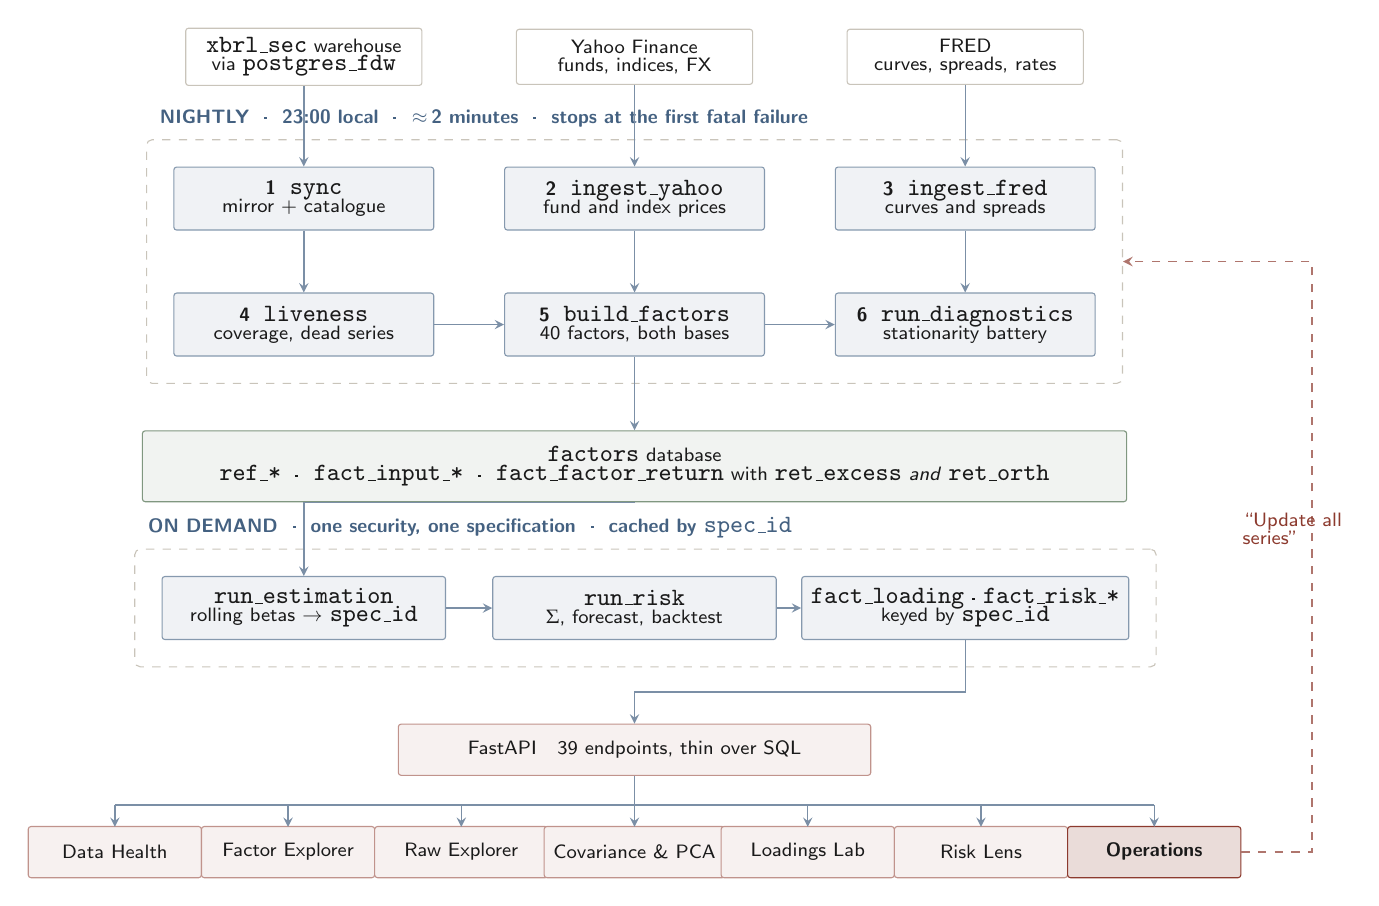
\begin{tikzpicture}[
  font=\sffamily\scriptsize,
  >=stealth,
  src/.style   = {draw=rule, fill=white, rounded corners=1pt, align=center,
                  minimum height=7mm, minimum width=30mm, text=ink},
  job/.style   = {draw=navy!55, fill=navy!7, rounded corners=1pt, align=center,
                  minimum height=8mm, minimum width=33mm, text=ink},
  store/.style = {draw=moss!70, fill=moss!8, rounded corners=1pt, align=center,
                  minimum height=9mm, minimum width=125mm, text=ink},
  ui/.style    = {draw=brick!55, fill=brick!7, rounded corners=1pt, align=center,
                  minimum height=6.5mm, minimum width=22mm, text=ink},
  lane/.style  = {draw=rule, dashed, rounded corners=2pt, inner sep=3.4mm},
  lbl/.style   = {font=\sffamily\scriptsize\bfseries, text=navy!85, anchor=west,
                  fill=white, inner xsep=2pt, inner ysep=1pt},
  flow/.style  = {->, draw=navy!60, line width=0.5pt},
  back/.style  = {->, draw=brick!70, line width=0.55pt, dashed},
]

% ---- sources (y = 0) --------------------------------------------------
\node[src] at (-42mm, 0)  (wh) {\code{xbrl\_sec} warehouse\\[-1.5pt]\scriptsize via \code{postgres\_fdw}};
\node[src] at (  0mm, 0)  (yh) {Yahoo Finance\\[-1.5pt]\scriptsize funds, indices, FX};
\node[src] at ( 42mm, 0)  (fr) {FRED\\[-1.5pt]\scriptsize curves, spreads, rates};

% ---- nightly chain (y = -18, -32) -------------------------------------
\node[job] at (-42mm, -18mm) (sync)  {\textbf{1} \ \code{sync}\\[-1.5pt]\scriptsize mirror + catalogue};
\node[job] at (  0mm, -18mm) (iy)    {\textbf{2} \ \code{ingest\_yahoo}\\[-1.5pt]\scriptsize fund and index prices};
\node[job] at ( 42mm, -18mm) (if)    {\textbf{3} \ \code{ingest\_fred}\\[-1.5pt]\scriptsize curves and spreads};
\node[job] at (-42mm, -34mm) (live)  {\textbf{4} \ \code{liveness}\\[-1.5pt]\scriptsize coverage, dead series};
\node[job] at (  0mm, -34mm) (build) {\textbf{5} \ \code{build\_factors}\\[-1.5pt]\scriptsize 40 factors, both bases};
\node[job] at ( 42mm, -34mm) (diag)  {\textbf{6} \ \code{run\_diagnostics}\\[-1.5pt]\scriptsize stationarity battery};

\begin{scope}[on background layer]
  \node[lane, fit=(sync)(iy)(if)(live)(build)(diag)] (nightly) {};
\end{scope}
\node[lbl] at ($(nightly.north west)+(1mm,2.6mm)$)
  {NIGHTLY \ · \ 23:00 local \ · \ $\approx$\,2 minutes \ · \ stops at the first fatal failure};

% ---- store (y = -52) --------------------------------------------------
\node[store] at (0mm, -52mm) (db)
  {\code{factors} database\\[-1pt]\scriptsize
   \code{ref\_*} \ · \ \code{fact\_input\_*} \ · \
   \code{fact\_factor\_return} with \code{ret\_excess} \emph{and} \code{ret\_orth}};

% ---- on demand (y = -70) ----------------------------------------------
\node[job, minimum width=36mm] at (-42mm, -70mm) (est)
  {\code{run\_estimation}\\[-1.5pt]\scriptsize rolling betas $\rightarrow$ \code{spec\_id}};
\node[job, minimum width=36mm] at (  0mm, -70mm) (risk)
  {\code{run\_risk}\\[-1.5pt]\scriptsize $\Sigma$, forecast, backtest};
\node[job, minimum width=36mm] at ( 42mm, -70mm) (cache)
  {\code{fact\_loading} · \code{fact\_risk\_*}\\[-1.5pt]\scriptsize keyed by \code{spec\_id}};

\begin{scope}[on background layer]
  \node[lane, fit=(est)(risk)(cache)] (ondemand) {};
\end{scope}
\node[lbl] at ($(ondemand.north west)+(1mm,2.6mm)$)
  {ON DEMAND \ · \ one security, one specification \ · \ cached by \code{spec\_id}};

% ---- serve ------------------------------------------------------------
\node[ui, minimum width=60mm] at (0mm, -88mm) (api)
  {FastAPI \ \ \scriptsize 39 endpoints, thin over SQL};

\node[ui] at (-66mm, -101mm) (p1) {Data Health};
\node[ui] at (-44mm, -101mm) (p2) {Factor Explorer};
\node[ui] at (-22mm, -101mm) (p3) {Raw Explorer};
\node[ui] at (  0mm, -101mm) (p4) {Covariance \& PCA};
\node[ui] at ( 22mm, -101mm) (p5) {Loadings Lab};
\node[ui] at ( 44mm, -101mm) (p6) {Risk Lens};
\node[ui, fill=brick!18, draw=brick] at (66mm, -101mm) (p7) {\textbf{Operations}};

% ---- edges ------------------------------------------------------------
\draw[flow] (wh) -- (sync);
\draw[flow] (yh) -- (iy);
\draw[flow] (fr) -- (if);
\draw[flow] (sync) -- (live);
\draw[flow] (iy) -- (build);
\draw[flow] (if) -- (diag);
\draw[flow] (live) -- (build);
\draw[flow] (build) -- (diag);
\draw[flow] (build.south) -- (db.north);

\draw[flow] (db.south) -| (est.north);
\draw[flow] (est) -- (risk);
\draw[flow] (risk) -- (cache);
\draw[flow] (cache.south) |- ($(api.north)+(0,4mm)$) -- (api.north);

% one bus from the API to the page row
\draw[draw=navy!60, line width=0.5pt] (api.south) -- (0mm,-95mm);
\draw[draw=navy!60, line width=0.5pt] (-66mm,-95mm) -- (66mm,-95mm);
\foreach \x in {-66,-44,-22,0,22,44,66}
  \draw[flow] (\x mm,-95mm) -- (\x mm,-97.8mm);

% the button that closes the loop, routed clear of everything on the right
\draw[back] (p7.east) -- ++(9mm,0) |- (nightly.east);
\node[font=\sffamily\scriptsize, text=brick, anchor=west, align=left]
  at (76mm, -60mm) {``Update all\\[-1.5pt]series''};

\end{tikzpicture}}
\caption{The terminal, end to end. Solid arrows are data flowing forward; the dashed
arrow is the Operations tab starting the nightly chain on request. The store in the
middle is the only state the two computation paths share, and it holds every factor
twice --- raw and orthogonalised --- which is what lets a specification name its own
panel and be scored against the matching covariance.}
\label{fig:flow}
\end{figure}

Three properties of that diagram are load-bearing.

\emph{The chain is ordered and fails closed.} Each stage is a prerequisite for the
ones after it, and the run stops at the first fatal failure rather than continuing
on half-refreshed inputs. A factor built on a partial refresh is worse than
yesterday's factor: it looks current and is not. Only the diagnostics stage is
advisory --- a warning on one factor should not stop a nightly run, and the
estimator reads the verdicts itself.

\emph{The store is the only shared state.} Nothing in the on-demand path calls
anything in the scheduled path, and neither calls the interface. A refresh that
fails leaves yesterday's panel intact and every cached specification still readable.

\emph{Both bases are stored, not derived.} \code{fact\_factor\_return} holds
\code{ret\_excess} and \code{ret\_orth} side by side. That is what allows a
specification to declare which panel it was estimated on and be scored against the
matching covariance (Section \ref{sec:bothpanels}).

\subsection{Updating every series, daily}
\label{sec:daily}

There are three ways to run the chain, and they run the same code.

\textbf{From the terminal's Operations tab.} A single button, \emph{Update all
series}. The six stages appear as a checklist that fills in as they complete, the
scheduler's own log streams underneath, and the page refuses to start a second run
while one is in flight. The tab also answers the question that comes before the
button: for each layer of the model --- instrument returns, level series, factor
returns --- it shows the newest observation and how many days behind the panel it
is, so that ``does this need refreshing?'' is visible rather than guessed.

\textbf{From the command line.} Identical work, identical exit code, and the exit
code is meaningful --- non-zero means a fatal stage failed, which is what makes it
safe to put behind a system scheduler.

\begin{lstlisting}
python -m backend.pipeline.scheduler --once
\end{lstlisting}

\textbf{As a daemon.} Runs the chain at 23:00 local: after the US close and the
FRED daily refresh, and before midnight so the run is stamped with the day whose
data it fetched.

\begin{lstlisting}
python -m backend.pipeline.scheduler
\end{lstlisting}

\begin{table}[htbp]
\centering
\caption{The nightly chain, with times from a representative run.}
\label{tab:chain}
\small
\begin{tabularx}{\textwidth}{@{}rlXr@{}}
\toprule
 & \textbf{Stage} & \textbf{What it does} & \textbf{Time} \\
\midrule
1 & \code{sync} & Mirrors warehouse prices over the foreign-data wrapper and
    rebuilds the 9{,}434-row security catalogue & 16s \\
2 & \code{ingest\_yahoo} & Total-return fund and index prices for every instrument
    a factor is built from & 20s \\
3 & \code{ingest\_fred} & Treasury curves, the ICE BofA spread ladder, policy rates,
    financial-conditions indices & 16s \\
4 & \code{liveness} & Recomputes each instrument's last observation, so the gate
    sees what the two ingests just fetched & 17s \\
5 & \code{build\_factors} & Constructs all forty factors on both bases & 14s \\
6 & \code{run\_diagnostics} & Stationarity battery over factors and instruments
    \emph{(advisory)} & 40s \\
\midrule
 & & \textbf{Total} & \textbf{$\approx$125s} \\
\bottomrule
\end{tabularx}
\end{table}

A \emph{full rebuild} --- also a button, also a flag (\code{--full}) --- ignores the
watermarks and re-fetches every history from the start. It is minutes rather than
seconds and is needed only after a schema change or a vendor restatement, which is
why it is the secondary control rather than the primary one.

\subsection{Estimating a security}

The on-demand path is reached from the Loadings Lab. Choosing a security and
pressing estimate does this:

\begin{enumerate}[leftmargin=1.6em,itemsep=0.35ex]
\item The parameters on the page hash to a \code{spec\_id}. If that identifier
  already has stored loadings, the response is a table read and the rest of this
  list does not happen.
\item If the security has never been priced here, it is pulled from the warehouse
  on the spot --- one indexed read --- and converted to the base currency.
\item The rolling regression runs: one fit per roll-forward step, each with its own
  diagnostics, stored against the \code{spec\_id}.
\item Requesting risk for that specification builds the covariance \emph{from the
  panel the specification names}, forecasts, scores the forecast against the
  forward outcome, and flags any window the reliability gate rejects.
\end{enumerate}

The catalogue behind step 2 is why the search box offers 9{,}434 securities rather
than the 203 the factor panel uses. It is materialised nightly by stage 1 because
deriving it live means aggregating two price tables of fifteen million rows apiece
--- around eight seconds per keystroke.

\subsection{What a refresh does not do}

Stated so that a green run is not read as more than it is. The chain refreshes
inputs and factors. It does not re-estimate loadings, does not re-score risk, and
does not back-fill a history a vendor has restated. The first two are on-demand by
design; the third is what the full rebuild is for. The Operations tab says all of
this on the page, next to the button, rather than in a document the person pressing
it has not read.

% =====================================================================
\section{Software architecture}
\label{sec:arch}

\subsection{The layering, and why it is the main design decision}

\begin{center}
\small
\begin{tabularx}{\textwidth}{@{}lXX@{}}
\toprule
\textbf{Layer} & \textbf{Contents} & \textbf{Constraint} \\
\midrule
\code{backend/core} & Statistics: 7 modules, 2{,}309 lines & Pure functions over arrays; no I/O \\
\code{backend/pipeline} & Ingestion, construction, estimation & May touch the database \\
\code{backend/app} & FastAPI routers, assistant & Thin; no statistics of its own \\
\code{sql} & 15 idempotent migrations & Applied in order, fail-fast \\
\code{frontend} & Next.js 14, seven pages & No computation beyond presentation \\
\bottomrule
\end{tabularx}
\end{center}

The \code{backend/core} boundary is the main architectural decision in the project.
Every statistical routine is a pure function over NumPy arrays with no database
access, no configuration lookup and no logging side effects. That is what makes the
accuracy claims in this paper checkable: a test can feed each routine a process whose
truth is known analytically and assert that it reaches the right answer, without a
database, a fixture or a network.

The alternative --- statistics computed inside the query that fetches the data, which
is the path of least resistance --- would make every claim in Sections
\ref{sec:orth} and \ref{sec:risk} unverifiable except by inspection.

\subsection{Data model}

The schema separates reference data (\code{ref\_}), facts (\code{fact\_}),
staging (\code{stage\_}), dimensions (\code{dim\_}) and operational state
(\code{etl\_}). The factor panel lives in one table with both bases side by side:

\begin{lstlisting}[language=SQL]
fact_factor_return(factor_id, date, ret_excess, ret_orth, ...)
\end{lstlisting}

Storing both columns rather than deriving one on read is what allows a specification
to name its panel and be scored consistently against it. Loadings, regression
diagnostics, covariance matrices, risk forecasts and backtests are all keyed by
\code{spec\_id} (Section \ref{sec:spec}), so the entire estimation for one set of
settings can be located, invalidated or recomputed as a unit.

Migrations are idempotent and applied in order by a fail-fast runner. The warehouse is
reached through \code{postgres\_fdw} rather than by copying: the security catalogue of
9{,}434 rows is materialised nightly, because deriving it live means aggregating two
price tables of fifteen million rows apiece --- around eight seconds per keystroke in
a search box.

\subsection{Pipeline jobs}

\begin{center}
\small
\begin{tabularx}{\textwidth}{@{}lX@{}}
\toprule
\code{sync} & Mirror the warehouse over the foreign-data wrapper; pull securities on demand \\
\code{ingest\_yahoo}, \code{ingest\_fred} & Refresh the factor universe and the level series \\
\code{build\_factors} & Construct all forty factors and both bases \\
\code{run\_diagnostics} & Run the stationarity battery over factors and instruments \\
\code{run\_estimation} & Rolling regression for one instrument under one specification \\
\code{run\_risk} & Covariance, forecast, backtest and reliability for one specification \\
\code{scheduler} & The nightly sequence, as one command \\
\bottomrule
\end{tabularx}
\end{center}

Each job writes an entry to an operational run log with its mode, scope and per-item
state, so a partial failure can be identified and resumed rather than re-run from the
beginning. The application surfaces this: selecting a run in the interface shows what
that run did, with its key parameters rendered as chips.

\subsection{API}

FastAPI over asyncpg, with the routers kept deliberately thin --- they translate
between HTTP and SQL and do no statistics. Thirty-nine endpoints across eight routers
cover factor series and diagnostics, raw source series, the covariance matrix and its
principal components, loadings estimation, risk, metadata, operations, and the
assistant.

The estimation endpoint is the one long-running call: a wide window rolled weekly is
upward of a thousand regressions, and the request does not return until every one is
written. The interface reports elapsed seconds rather than a static spinner, because a
motionless ``Estimating\dots'' for half a minute is indistinguishable from a hung
page.

\subsection{Interface}

Seven pages --- Data Health, Factor Explorer, Raw Explorer, Covariance \& PCA,
Loadings Lab, Risk Lens and Operations --- on Next.js 14 with Plotly for charts.
Section \ref{sec:workflow} describes what the last of them is for. Three conventions
run through all the others.

\paragraph{Colour is a claim, not decoration.} Colour on a diagnostic says whether the
number is what the model wants, and the rule lives in a single module so that two
pages cannot colour the same $p$-value differently. There are three tones and the
third carries the weight: green where the test says what we want, amber where it flags
something nothing is gated on, and plain where the outcome is expected. A rejected
ARCH-LM or Jarque-Bera test is never red --- volatility clustering and fat tails are
the normal condition of a daily return series. Only the joint ADF\,$\times$\,KPSS
verdict, a wrong VaR breach count, and a design past the condition-number limit earn
red.

\paragraph{Every metric explains itself.} Each headline figure is a card that, on
hover, states what the metric is, how it is computed and how to read it. The intent is
that a number never appears without its definition being one gesture away.

\paragraph{Provenance is visible.} The Raw Explorer shows the source system, the
original vendor label and the full available history for every series, alongside the
Python that turns it into a factor --- extracted from the live source at request time,
so it cannot fall out of date with the code that runs.

\subsection{The assistant}

An optional panel answers questions about the methodology and about the numbers
currently on screen. It is grounded two ways: a methodology corpus assembled at
startup from the module docstrings in \code{backend/core} and the registry note on
every factor, and a snapshot of exactly what the open page has rendered.

It has no tools and no database access of its own, which is deliberate. The system
prompt makes the supplied figures authoritative over the model's own arithmetic, so
when asked for something not in view it names the page that produces it rather than
estimating. Three live tests hold it to that contract.

\subsection{Testing}
\label{sec:testing}

The suite is 352 tests. They do not check that functions return numbers; each feeds a
statistical routine a process whose truth is known and asserts that it reaches the
right conclusion:

\begin{itemize}[leftmargin=1.4em,itemsep=0.3ex]
\item a random walk must fail the stationarity gate; an AR(1) with $\phi=0.5$ must pass
\item a GARCH series must flag ARCH effects \emph{without} failing
\item a smoothed series must show a variance ratio above 1
\item a forecast at half the true volatility must produce a bias statistic of 2
\item clustered VaR breaches must be caught by Christoffersen even where Kupiec sees
  nothing wrong with the count
\item shrinkage must beat the sample covariance when factors outnumber observations
\item every rendered factor formula, evaluated independently, must reproduce the
  builder's output
\end{itemize}

This approach earned its keep. Five defects were found by tests or diagnostics rather
than by inspection, and each would have silently corrupted results:

\begin{enumerate}[leftmargin=1.6em,itemsep=0.35ex]
\item The variance-ratio implementation in the \code{arch} package consumes a
  \emph{price level} and differences internally. Passing returns differenced twice,
  giving $\mathrm{VR}\approx 1/q$ and flagging every clean factor as mean-reverting.
\item The ridge penalty was scaled by $\sigma^{-2}$ instead of $\sigma^{2}$, so
  $\lambda = 1$ shrank every loading to zero.
\item Crypto weekend prints polluted the trading calendar, cutting the covariance
  matrix from 39 factors to 8.
\item \code{fx\_carry} was the yen short wearing another name --- correlation $-0.87$
  with \code{fx\_jpy} before it was residualised against it.
\item Stability columns held IEEE NaN rather than NULL, because pandas converts
  \code{None} to NaN in a float column and \code{double precision} accepts it.
  \code{IS NULL} never matched, \code{count()} counted them, and a single NaN turned
  an average over the whole column into NaN.
\end{enumerate}

None of the five would have raised an error. Each produced a plausible number.

\subsection{Operations and reproducibility}

The nightly refresh is a single command. A launcher script starts the API and the web
application, waits until both answer, and opens the browser; anything already serving
is left alone. It carries one non-obvious check. A production Next.js server reads its
build manifest once, at boot, so rebuilding the frontend while it runs leaves it
serving HTML that points at the previous build's hashed chunks. Those files no longer
exist, so the assets 404 --- a missing stylesheet renders the page as unstyled HTML, a
missing script renders nothing at all, and neither reports anything. Port-probing
cannot detect it, because the server answers 200 perfectly well. The script therefore
requests every route's HTML, follows every asset each one references, and restarts the
web application when any of them fails to resolve; the route list is read from the
prerendered pages on disk, so adding a page cannot leave it unchecked.

% =====================================================================
\section{Limits}
\label{sec:limits}

\begin{description}[leftmargin=1.6em,style=nextline,itemsep=0.45ex]
\item[Style proxies are long-only funds.] Not long-short portfolios. Validated
  correlations after orthogonalisation: momentum 0.64, value 0.50, low volatility
  0.20, quality 0.14. The last two are weak and should not be leaned on.
\item[FX carry is an approximation.] Three policy-rate differentials in place of a
  G10 basket built from forward points, with a residual yen dependence of $+0.16$
  after residualisation.
\item[Euro-area and Japanese rates lag.] They are warehouse-sourced with no refresh in
  this project.
\item[Short histories.] Style factors begin in 2011--2013 and \code{liq\_funding} in
  2018. Any window longer than the shortest factor's history silently drops it; the
  usable factor count is recorded per window for this reason.
\item[Breach clustering is unresolved.] Both panels fail Christoffersen. Applying a
  21-day-horizon forecast to daily returns produces dependent exceptions by
  construction, and the honest description is that the horizon and the test are
  mismatched rather than that the model passes.
\item[No optimiser, no attribution, no macro state space.] See below.
\item[The model can only measure risks that have appeared in returns.] Derivatives,
  concentration and tail positions remain invisible. This is why specific risk has a
  floor and why model uncertainty is surfaced rather than hidden.
\end{description}

Three components a factor model of this kind is often expected to carry are absent
deliberately rather than by oversight.

\emph{Portfolio optimisation and performance attribution.} The covariance matrix is
optimiser-ready --- positive semi-definite, with interpretable exposures --- but no
optimiser sits on top of it, and no attribution layer decomposes a realised return
into factor contributions. Both are downstream consumers of the model rather than
parts of it, and building either before the risk forecast has been shown to be right
would be building on an unverified base.

\emph{A mixed-frequency state-space layer.} Macro release surprises are implemented
only as the sparse release-event transform of Section \ref{sec:data}. There is no
announcement-window lead-lag structure and no Kalman-filtered latent macro state
interpolating releases onto a daily grid. Interpolation is exactly the forward fill
this model refuses elsewhere, with a filter in front of it; doing it properly means
committing to a state equation that the data available here cannot identify.

% =====================================================================
% =====================================================================
%  Appendices. Included by factor-model-paper.tex.
% =====================================================================
\appendix
\newpage

\section{Statistical methodology}
\label{app:method}

This appendix states each procedure in the form in which it is implemented, including
the conventions --- bandwidth rules, degrees of freedom, boundary handling --- that
decide whether two nominally identical implementations agree. Every routine named
here is a pure function over arrays in \code{backend/core} and is exercised by the
test suite against a process whose answer is known analytically.

\subsection{Conventions}

The significance level is $\alpha = 0.05$ throughout, and every $p$-value is stored
and displayed so that a reader may disagree with the threshold. Returns are natural
logarithms. Annualisation uses 252 trading days: a daily standard deviation is
multiplied by $\sqrt{252}$ and a daily mean by 252. Sample standard deviations use
$\mathrm{ddof}=1$ unless stated; the Ledoit-Wolf derivation is the exception and is
noted where it arises.

% ---------------------------------------------------------------------
\subsection{The stationarity battery}
\label{app:stationarity}

A single Dickey-Fuller test is useless as a gate on daily returns: it rejects almost
always, so it cannot discriminate. The battery is therefore built around what
actually goes wrong with financial series --- an untransformed level, a structural
break, stale pricing, illiquidity --- with each test given the role its own null
hypothesis supports.

\subsubsection{Unit-root tests, read jointly}

\begin{description}[leftmargin=1.6em,style=nextline,itemsep=0.35ex]
\item[Augmented Dickey-Fuller \citep{dickey1979}.] $H_0$: a unit root is present. Lag
  order is selected by AIC; the regression includes a constant, which is the right
  specification for an excess return with a possible non-zero mean.
\item[KPSS \citep{kpss1992}.] $H_0$: the series \emph{is} stationary --- the exact
  complement of ADF. Level stationarity, with the automatic Newey-West bandwidth.
\item[Phillips-Perron \citep{phillips1988}.] Same null as ADF but with a
  non-parametric correction for serial correlation and heteroskedasticity in place of
  ADF's augmentation lags. Reported alongside as a robustness check, not gated on.
\end{description}

ADF and KPSS have opposite nulls, and reading them together yields four verdicts where
either alone yields two. This is the single most useful idea in the battery:

\begin{table}[htbp]
\centering
\small
\caption{Joint reading of ADF and KPSS at $\alpha = 0.05$.}
\begin{tabular}{@{}llll@{}}
\toprule
\textbf{ADF} & \textbf{KPSS} & \textbf{Verdict} & \textbf{Consequence} \\
\midrule
rejects & does not reject & stationary & pass \\
does not reject & rejects & \textbf{unit root} & \textbf{fail} --- must be differenced \\
rejects & rejects & break or heteroskedasticity & warn \\
does not reject & does not reject & inconclusive --- usually too short & warn \\
\bottomrule
\end{tabular}
\end{table}

Only the second row blocks a series. The third is the interesting one: both tests
rejecting is not a contradiction but a signature --- it indicates a structural break or
strong heteroskedasticity rather than a clean unit root, and it is the only condition
under which the Zivot-Andrews test is run.

\subsubsection{Structural break}

\textbf{Zivot-Andrews \citep{zivot1992}} tests a unit root against stationarity around
a single endogenously determined break, searching every candidate break date and
taking the minimum statistic. It is by far the most expensive test in the battery,
which is why it runs only when the joint reading says ``not a clean unit root'' and at
least 100 observations are available. The estimated break date is stored, because a
break in 2008-09 and a break in 2020-03 invite different conclusions.

\subsubsection{Stale pricing}

\textbf{Lo-MacKinlay variance ratio \citep{lo1988}}, heteroskedasticity-robust, at
lags $q \in \{2,5,10\}$:

\begin{equation}
\mathrm{VR}(q) \;=\; \frac{\operatorname{Var}\!\left(\sum_{j=0}^{q-1} r_{t-j}\right)}{q \operatorname{Var}(r_t)} .
\end{equation}

Under a random walk $\mathrm{VR}=1$. Values above 1 indicate positive autocorrelation
--- trending or smoothed pricing --- and values below 1 mean reversion. The
heteroskedasticity-robust variant is essential: daily returns are conditionally
heteroskedastic by construction, and the homoskedastic version rejects on that alone.

\begin{decision}{A level, not a return}
The \code{arch} package's variance-ratio implementation consumes a \emph{price level}
and differences internally. Passing returns to it differences twice, giving
$\mathrm{VR} \approx 1/q$ and flagging every clean factor as mean-reverting. The
implementation here therefore reconstructs a level by cumulative summation before
calling it, and a test asserts that a smoothed series shows $\mathrm{VR} > 1$ --- which
is how the defect was found.
\end{decision}

\textbf{Ljung-Box \citep{ljung1978}} at 10 lags, $H_0$: no autocorrelation up to lag
10. It is the second stale-pricing signal, and is also computed on squared returns,
where rejection indicates volatility clustering rather than predictability in the mean.

\subsubsection{Conditional heteroskedasticity}

\textbf{Engle's ARCH-LM \citep{engle1982}} at 10 lags, $H_0$: no conditional
heteroskedasticity. \emph{This test is recorded and never gated on.} A GARCH process
is strictly stationary; gating on ARCH-LM would exclude essentially every financial
series ever published. The reason to know about clustering is that it argues for HAC
standard errors --- not against the factor.

\subsubsection{Distribution and liquidity}

Skewness, excess kurtosis (Fisher convention, zero for a Gaussian) and the
Jarque-Bera statistic are recorded. Like ARCH-LM, Jarque-Bera is never gated on: fat
tails are the normal condition of a daily return series.

The \textbf{zero-return share} is the cheapest and frequently the most telling check in
the battery. Above 50\% the series is not really trading daily and the verdict fails;
above 20\% it warns. The \textbf{maximum absolute return} is recorded as a
data-integrity check --- a single print of $-5.775$ in log space is not a market event
but a corporate action or a bad first row.

\subsubsection{Verdict assembly}

\begin{center}
\small
\begin{tabular}{@{}lll@{}}
\toprule
\textbf{Condition} & \textbf{Verdict} & \textbf{Flag} \\
\midrule
Joint reading is ``unit root'' & fail & \code{unit\_root} \\
Fewer than 60 observations & fail & \code{too\_short} \\
Zero variance & fail & \code{constant} \\
Zero-return share $> 0.50$ & fail & \code{illiquid} \\
\addlinespace
Joint reading inconclusive & warn & \code{inconclusive\_unit\_root} \\
Joint reading is ``break'' & warn & \code{structural\_break} \\
Fewer than 252 observations & warn & \code{short\_history} \\
Zero-return share $> 0.20$ & warn & \code{sparse\_trading} \\
$|\mathrm{VR}-1| > 0.25$ with a significant $p$ & warn & \code{stale\_pricing} \\
\bottomrule
\end{tabular}
\end{center}

Every flag carries a human-readable reason, and the reason rather than the flag is
what the interface displays.

\subsubsection{Sparse release factors}

A release-event factor is zero on roughly 80\% of days by construction. The liquidity
and stale-pricing gates would read that as a dead instrument. For a series marked
sparse, the tests therefore run on the non-zero subsequence --- the statistically
meaningful object is the sequence of releases --- and the sparsity is reported rather
than penalised. A short window over such a factor holds few releases, so it warns
instead of failing, with the reason directing the reader to the full-history
diagnostic where power is adequate.

% ---------------------------------------------------------------------
\subsection{Regression}
\label{app:regression}

\subsubsection{Weighted least squares}

With design matrix $X$ (a column of ones followed by the factor panel) and weights $w$
normalised to mean one, the estimator solves the weighted normal equations. Equal
weighting sets $w_t = 1$; exponential weighting sets

\begin{equation}
w_t \;\propto\; 2^{-(T-t)/H},
\end{equation}

for half-life $H$ in days, again normalised to mean one so that the effective sample
size is comparable across settings.

\subsubsection{Huber}

Robust regression \citep{huber1964} by iteratively reweighted least squares, five
iterations, with tuning constant $\delta = 1.345$ --- the value giving 95\% asymptotic
efficiency under Gaussian errors. The weight function is

\begin{equation}
\psi(z) \;=\; \begin{cases} 1 & |z| \le \delta \\ \delta/|z| & |z| > \delta\end{cases},
\qquad z_t = \frac{\varepsilon_t}{\hat s},
\end{equation}

with $\hat s$ a robust scale estimate of the residuals. Observations inside $\delta$
robust standard deviations keep unit weight; those outside are downweighted in
proportion to their distance rather than discarded.

\subsubsection{Ridge}
\label{app:ridge}

The penalty applies to standardised slopes so that $\lambda$ does not depend on
whether a factor is quoted in percent or in decimals, and the intercept is left
unpenalised so that $\alpha$ is not biased toward zero. Penalising
$\sum_j (b_j \sigma_j)^2$ gives normal equations

\begin{equation}
\left(X^{\prime}X + \lambda n \operatorname{diag}(\sigma^2)\right) b \;=\; X^{\prime}y ,
\end{equation}

so the penalty is \emph{multiplied} by $\sigma^2$.

\begin{decision}{The sign of an exponent}
The original implementation divided by $\sigma^2$ instead. For daily returns with
$\sigma \approx 0.01$ that inflates the penalty by a factor of $10^4$, and $\lambda=1$
shrank every loading to exactly zero. The regression still returned, still reported an
$R^2$, and still produced a loading vector; it was simply the zero vector. A test that
asserts a modest ridge penalty leaves a known loading recognisable is what caught it.
\end{decision}

\subsubsection{HAC standard errors}

Newey-West \citep{newey1987} with Bartlett (triangular) weights:

\begin{equation}
V \;=\; (X^{\prime}X)^{-1}\left[S_0 + \sum_{\ell=1}^{L} w_\ell\left(\Gamma_\ell + \Gamma_\ell^{\prime}\right)\right](X^{\prime}X)^{-1},
\qquad w_\ell = 1 - \frac{\ell}{L+1},
\end{equation}

where $\Gamma_\ell$ is the lag-$\ell$ autocovariance of the score vectors
$\varepsilon_t x_t$. Bartlett weights guarantee a positive semi-definite result, which
a truncated (unweighted) kernel does not. The automatic bandwidth is

\begin{equation}
L \;=\; \left\lfloor 4\left(\frac{T}{100}\right)^{2/9} \right\rfloor ,
\end{equation}

giving 4 lags at 100 observations, 5 at 252 and 6 at 1000. The bandwidth is
deliberately small: autocorrelation in daily returns is short-lived, and the cost of
over-specifying $L$ is a noisy covariance estimate.

\subsubsection{Dimson lead-lag}

The design is augmented with $L$ lagged copies of the factor panel and the
coefficients are summed factor by factor (Section \ref{sec:dimson}). Only lags are
included; a lead would use tomorrow's factor return to explain today's security
return, which is unavailable at forecast time.

The standard error of the sum uses the full coefficient covariance:

\begin{equation}
\operatorname{se}\!\left(\hat\beta^{\mathrm{Dimson}}_j\right)
= \sqrt{\textstyle\sum_{\ell}\sum_{m} \operatorname{Cov}\!\left(\hat\beta^{(\ell)}_j, \hat\beta^{(m)}_j\right)} .
\end{equation}

The lag coefficients are typically negatively correlated, so the diagonal-only
approximation $\sqrt{\sum_\ell \operatorname{se}^2}$ overstates the uncertainty. It is
used only as a conservative fallback when no covariance is supplied, and the caller is
told to treat the resulting interval as wide.

\subsubsection{Collinearity diagnostics}

The \textbf{condition number} is the ratio of the largest to the smallest singular
value of the standardised design matrix. It is the invariant that governs how far
$\beta^{\prime}\Sigma\beta$ can be amplified by near-collinearity, and it is what the
reliability gate of Section \ref{sec:reliability} reads.

\textbf{Variance inflation factors} are computed from the inverse correlation matrix,

\begin{equation}
\mathrm{VIF}_j \;=\; \left[R^{-1}\right]_{jj},
\qquad R = \operatorname{corr}(X),
\end{equation}

which is algebraically identical to $1/(1-R_j^2)$ from $k$ auxiliary regressions but
costs one matrix inversion rather than $k$ least-squares fits --- a material difference
at $k=40$ over a thousand rolling windows. The auxiliary-regression form is retained
in the code as the reference implementation, and a test asserts the two agree.

\subsubsection{Beta stability}

Between consecutive windows, on the factors common to both:

\begin{equation}
d_{L_1} = \sum_{j \in C} \left|\beta_j^{(t)} - \beta_j^{(t-1)}\right|,
\qquad
\rho = \operatorname{corr}\!\left(\beta^{(t)}_C, \beta^{(t-1)}_C\right),
\qquad |C| \text{ recorded.}
\end{equation}

Recording $|C|$ is not optional: $d_{L_1}$ falls mechanically as the common basis
narrows, so the two must be read together.

% ---------------------------------------------------------------------
\subsection{Orthogonalisation}
\label{app:orth}

Given a target series $y$ and a regressor block $X$ drawn from the levels above it in
the hierarchy, the rolling residual is computed as follows.

\begin{enumerate}[leftmargin=1.6em,itemsep=0.3ex]
\item Coefficients are refitted at $t$ whenever $t$ has reached the next refit point,
  on the trailing window $[\max(0,\,t-504),\,t)$, requiring at least
  $\max(252,\ k+2)$ complete observations. The window is half-open: the fit uses data
  strictly before $t$.
\item The next refit point is set to $t + 21$.
\item The residual at $t$ is $y_t - \hat a - \hat b^{\prime}X_t$, using whichever
  coefficients are currently in force.
\item Before the first successful fit, the residual is undefined rather than equal to
  the raw series --- a factor's orthogonalised history starts when it can be
  estimated, not before.
\end{enumerate}

Two variants exist for comparison and are exercised by the test suite: an expanding
window, and an exact full-sample fit. Table \ref{tab:causal} reports what each costs.
The full-sample variant is the only one that achieves exact orthogonality, and it is
the only one that uses future information; it is never used to build the panel.

A Gram-Schmidt routine is also available, which orthogonalises a panel's columns
sequentially left to right. It is used for diagnostics rather than construction,
because the block hierarchy --- not column order --- is what encodes the economic
argument about which factor should absorb shared variation.

% ---------------------------------------------------------------------
\subsection{Covariance estimation}
\label{app:cov}

\subsubsection{Sample}

The unbiased sample covariance on complete rows, annualised by 252. Included as a
baseline and as the reference against which shrinkage is tested; it is not a
sensible choice at $K=39$ on a rolling window.

\subsubsection{Exponentially weighted}

RiskMetrics-style, with weights $w_t \propto 2^{-(T-t)/H}$ normalised to sum to one
and a default half-life of $H=60$ days. Two details matter.

Deviations are taken from the \emph{weighted} mean rather than the simple mean, so
the estimate is internally consistent. And the result is bias-corrected for weighted
sampling,

\begin{equation}
\hat\Sigma = \frac{\sum_t w_t (x_t-\bar x_w)(x_t-\bar x_w)^{\prime}}{1 - \sum_t w_t^2},
\end{equation}

since $1/\sum_t w_t^2$ is the effective sample size when the weights sum to one.

\begin{decision}{Sixty days, not eleven}
The classic RiskMetrics $\lambda = 0.94$ corresponds to a half-life of about 11 days.
That is too jumpy for a risk model used to set limits: the forecast moves materially
on a single day's return. Sixty days is the usual compromise and is the default here.
\end{decision}

\subsubsection{Ledoit-Wolf shrinkage}

Shrinkage toward a \emph{constant-correlation} target \citep{ledoit2003}. The target
$F$ keeps each factor's own variance and replaces every correlation by the average
correlation $\bar r$:

\begin{equation}
F_{ij} = \bar r\, s_i s_j \;\; (i \neq j), \qquad F_{ii} = s_i^2 .
\end{equation}

This is a considerably better description of a factor panel than the identity target
used in the simpler version of the method, which asserts that the factors are
uncorrelated --- precisely the assumption a factor panel violates.

The optimal intensity is

\begin{equation}
\delta^{\star} = \max\!\left\{0,\ \min\!\left\{1,\ \frac{\pi - \rho}{\gamma}\cdot\frac{1}{T}\right\}\right\},
\qquad \hat\Sigma = \delta^{\star} F + (1-\delta^{\star}) S,
\end{equation}

where $\pi$ is the summed asymptotic variance of the sample covariance entries, $\rho$
the asymptotic covariance between the target's estimation error and the sample's, and
$\gamma = \|F - S\|_F^2$ the squared misspecification of the target. The derivation
assumes the maximum-likelihood scaling for $S$ (divisor $T$), which is what the
implementation uses internally; the result is converted to the unbiased scaling
(divisor $T-1$) before being returned, so that it is directly comparable with the
sample estimator. The realised $\delta^{\star}$ is stored on the result --- it is
informative in itself, since a high intensity says the sample estimate was carrying
little signal.

\subsubsection{Blend}

$\Sigma = a\,\Sigma_{\mathrm{EWMA}} + (1-a)\,\Sigma_{\mathrm{shrunk}}$, default
$a = 0.6$. The EWMA leg supplies responsiveness to the current regime; the shrunk leg
supplies conditioning. This is the default estimator.

\subsubsection{Positive semi-definiteness}

Every estimate is checked. Where the smallest eigenvalue is negative, the matrix is
repaired by clipping eigenvalues at a small positive floor and reconstructing, then
\emph{rescaled} so that the diagonal returns to the original factor variances.

The rescale is the part that is easy to omit and important to keep: clipping alone
raises the diagonal, which raises every volatility computed from the matrix. The
repair is recorded on the result rather than applied silently.

\subsubsection{Specific risk}

\begin{equation}
\sigma^2_\varepsilon \;=\; \max\!\left\{\sigma^2_{\mathrm{floor}},\;
(1-k)\,\mathrm{EWMA}_H\!\left[\varepsilon_t^2\right] \cdot 252 \;+\; k\,\sigma^2_{\mathrm{peer}}\right\},
\end{equation}

with $H = 60$ days, $k = 0.25$, and $\sigma_{\mathrm{floor}} = 2\%$ annualised. The
peer variance is the cross-sectional median residual volatility across every
instrument estimated under the same specification, squared. Both the raw and the
floored values are returned, along with a flag recording whether the floor bound,
so that a floored number is never mistaken for a measured one.

\subsubsection{Assembly and attribution}

\begin{equation}
\Sigma_r = B\,\Sigma_F\,B^{\prime} + \operatorname{diag}(\sigma^2_\varepsilon),
\qquad
\sigma_p = \sqrt{\beta^{\prime}\Sigma_F\beta + \sigma^2_\varepsilon} .
\end{equation}

Risk contributions use the standard Euler decomposition,
$\mathrm{RC}_j = \beta_j\,(\Sigma_F\beta)_j / \sigma_p$, which sums to the factor part
of total risk exactly. Contributions are aggregated to block level for display,
because a forty-row contribution table is not a decomposition anyone reads.

% ---------------------------------------------------------------------
\subsection{Forecast evaluation}
\label{app:eval}

\subsubsection{Realised volatility and alignment}

For horizon $h$, realised volatility at $t$ is the annualised standard deviation of
$r_{t+1},\dots,r_{t+h}$. The forecast it is compared against uses loadings from a
window ending at or before $t$ and a covariance estimated on returns up to $t$. The
forward window is constructed by an explicit shift rather than by a rolling operation
with a default alignment, because an off-by-one in this direction is lookahead and
produces a flatteringly good result.

\subsubsection{Bias statistics}

Two are computed. The \textbf{mean bias ratio} is
$\overline{\sigma^{\mathrm{real}}/\sigma^{\mathrm{pred}}}$; it is intuitive but noisy,
being a ratio of volatilities and therefore right-skewed. The \textbf{bias statistic}
is the sharper and is what the text quotes:

\begin{equation}
z_t = \frac{r_t}{\sigma^{\mathrm{pred}}_t},
\qquad
\mathrm{bias} = \operatorname{sd}(z_t),
\end{equation}

the standard deviation of returns divided by the volatility forecast in force at
each date. It equals 1 when the model is calibrated and exceeds 1 when risk is
underestimated. The kurtosis of $z$ is recorded alongside it: a bias statistic of 1
with a kurtosis of 8 describes a model that is right on average and wrong in the
tails.

\subsubsection{Mincer-Zarnowitz}

Realised variance regressed on predicted variance \citep{mincer1969}:

\begin{equation}
\left(\sigma^{\mathrm{real}}_t\right)^2 = a + b\left(\sigma^{\mathrm{pred}}_t\right)^2 + u_t,
\qquad H_0:\ (a,b) = (0,1).
\end{equation}

Run on variances rather than volatilities, because variance is what the model
forecasts and what aggregates linearly. Individual $t$-tests for $a=0$ and $b=1$ are
reported together with a joint Wald test,
$W = (\hat\theta - \theta_0)^{\prime} V^{-1} (\hat\theta - \theta_0) \sim \chi^2_2$.

HAC standard errors are not optional here. Overlapping realised windows --- a 21-day
forward window observed daily --- induce strong serial correlation in $u_t$ by
construction, and ordinary standard errors would reject far too often. Section
\ref{sec:risk} gives the separate caveat on interpreting the slope.

\subsubsection{Value at risk and expected shortfall}

\begin{equation}
\mathrm{VaR}_t(\alpha) = -z_\alpha\,\frac{\sigma^{\mathrm{pred}}_t}{\sqrt{252}},
\end{equation}

under either a Gaussian quantile or a scaled Student-$t$ quantile with 5 degrees of
freedom, the latter being the more honest default for daily returns. Expected
shortfall is computed at the 97.5\% level under the same distributional choice.

\subsubsection{Kupiec proportion of failures}

\citep{kupiec1995} A likelihood ratio on the exception \emph{count}, $\chi^2_1$:

\begin{equation}
\mathrm{LR}_{\mathrm{POF}} = -2\left[(T-x)\log(1-p) + x\log p - (T-x)\log(1-\hat\pi) - x\log\hat\pi\right],
\end{equation}

with $p = 1-\alpha$, $x$ exceptions in $T$ observations and $\hat\pi = x/T$. At the
boundaries $x = 0$ or $x = T$ the ratio is degenerate; the implementation falls back
to an exact two-sided binomial probability rather than returning a spurious statistic.

\subsubsection{Christoffersen conditional coverage}

\citep{christoffersen1998} $H_0$: the correct rate \emph{and} independence.
Transitions are counted as $n_{ij}$ (from state $i$ to state $j$, breach = 1), and

\begin{equation}
\mathrm{LR}_{\mathrm{CC}} = \mathrm{LR}_{\mathrm{POF}} + \mathrm{LR}_{\mathrm{IND}} \sim \chi^2_2 .
\end{equation}

Where the transition counts cannot identify the independence term --- no breach ever
follows a non-breach, or one of the states is never visited --- the implementation
reports Kupiec alone on one degree of freedom rather than pretending to test
something the data cannot support.

This is the test that matters most and is reported even when it fails, because
clustered breaches are the dangerous failure: a model can produce exactly the right
number of exceptions over a decade and place them all in one week.

% ---------------------------------------------------------------------
\subsection{Density estimation}
\label{app:density}

The distribution panel exists to answer one question --- how far from Gaussian is this
series, and where --- so its defaults are chosen to keep the tails visible rather than
to produce a smooth picture.

\paragraph{Robust scale.} The smaller of the sample standard deviation and
$\mathrm{IQR}/1.349$. The two coincide for a Gaussian sample; on a fat-tailed series
the second is much smaller, and taking the minimum ties bandwidth and bin width to the
bulk of the distribution, which is where resolution is wanted.

\paragraph{Bin count.} Freedman-Diaconis \citep{freedman1981},
$h = 2\,\mathrm{IQR}\,n^{-1/3}$, with the resulting count clamped to $[20, 220]$ for
legibility. Scott's rule uses the standard deviation and would be inflated by exactly
the outliers that create the problem.

\paragraph{Bandwidth.} Silverman's rule \citep{silverman1986} on the robust scale,
$h = 0.9\,s\,n^{-1/5}$. Using the plain standard deviation here over-smooths a
fat-tailed series into a flat blob.

\paragraph{Overlays and range.} A Gaussian fit and a Student-$t$ fit are drawn over
the empirical density; the comparison between them is the whole purpose of the panel.
The drawing range is the 0.1st to 99.9th percentile, and the observations outside it
are \emph{counted and reported}, not silently dropped --- a plot that hid its own tail
would be worse than the naive one it replaces.

\newpage
% =====================================================================
\section{Factor registry}
\label{app:registry}

The forty factors, their block, their hierarchy level and the factors each is
residualised against. Level 0 factors are used raw. A factor's orthogonalisation
targets are always factors at a lower level, so the hierarchy is acyclic by
construction and the panel can be built in one pass.

The construction of each factor --- the exact formula over named instruments --- is
given in the companion document \emph{factor-formulas}, which is generated from this
same registry.

% Generated by scripts/build_paper.py — do not edit by hand.
\begingroup\small
\setlength{\LTleft}{0pt}\setlength{\LTright}{\fill}
\begin{longtable}{@{}llc>{\raggedright\arraybackslash}p{0.40\textwidth}@{}}
\toprule
\textbf{Factor} & \textbf{Block} & \textbf{Level} & \textbf{Residualised against} \\
\midrule
\endfirsthead
\toprule
\textbf{Factor} & \textbf{Block} & \textbf{Level} & \textbf{Residualised against} \\
\midrule
\endhead
\bottomrule
\endfoot
\texttt{\footnotesize eq\_global} & Equity Market & 0 & \textit{--- used raw} \\
\texttt{\footnotesize eq\_cyclical} & Equity Market & 1 & \texttt{\footnotesize eq\_global} \\
\texttt{\footnotesize eq\_em} & Equity Market & 1 & \texttt{\footnotesize eq\_global} \\
\texttt{\footnotesize eq\_europe} & Equity Market & 1 & \texttt{\footnotesize eq\_global} \\
\texttt{\footnotesize eq\_japan} & Equity Market & 1 & \texttt{\footnotesize eq\_global} \\
\texttt{\footnotesize eq\_size} & Equity Market & 1 & \texttt{\footnotesize eq\_global} \\
\texttt{\footnotesize eq\_us} & Equity Market & 1 & \texttt{\footnotesize eq\_global} \\
\addlinespace
\texttt{\footnotesize sty\_lowvol} & Equity Style & 2 & \texttt{\footnotesize eq\_global}, \texttt{\footnotesize eq\_us}, \texttt{\footnotesize eq\_cyclical} \\
\texttt{\footnotesize sty\_momentum} & Equity Style & 2 & \texttt{\footnotesize eq\_global}, \texttt{\footnotesize eq\_us}, \texttt{\footnotesize eq\_cyclical} \\
\texttt{\footnotesize sty\_quality} & Equity Style & 2 & \texttt{\footnotesize eq\_global}, \texttt{\footnotesize eq\_us}, \texttt{\footnotesize eq\_cyclical} \\
\texttt{\footnotesize sty\_value} & Equity Style & 2 & \texttt{\footnotesize eq\_global}, \texttt{\footnotesize eq\_us}, \texttt{\footnotesize eq\_cyclical} \\
\addlinespace
\texttt{\footnotesize rt\_breakeven} & Rates & 0 & \texttt{\footnotesize rt\_us\_level} \\
\texttt{\footnotesize rt\_ea\_level} & Rates & 0 & \texttt{\footnotesize rt\_us\_level} \\
\texttt{\footnotesize rt\_jp\_level} & Rates & 0 & \texttt{\footnotesize rt\_us\_level} \\
\texttt{\footnotesize rt\_uk} & Rates & 0 & \texttt{\footnotesize rt\_us\_level} \\
\texttt{\footnotesize rt\_us\_curve} & Rates & 0 & \textit{--- used raw} \\
\texttt{\footnotesize rt\_us\_level} & Rates & 0 & \textit{--- used raw} \\
\texttt{\footnotesize rt\_us\_slope} & Rates & 0 & \textit{--- used raw} \\
\addlinespace
\texttt{\footnotesize cr\_em\_hard} & Credit & 1 & \texttt{\footnotesize rt\_us\_level}, \texttt{\footnotesize rt\_us\_slope}, \texttt{\footnotesize cr\_hy}, \texttt{\footnotesize eq\_global} \\
\texttt{\footnotesize cr\_hy} & Credit & 1 & \texttt{\footnotesize rt\_us\_level}, \texttt{\footnotesize rt\_us\_slope}, \texttt{\footnotesize eq\_global} \\
\texttt{\footnotesize cr\_ig} & Credit & 1 & \texttt{\footnotesize rt\_us\_level}, \texttt{\footnotesize rt\_us\_slope} \\
\texttt{\footnotesize cr\_loans} & Credit & 1 & \texttt{\footnotesize rt\_us\_level}, \texttt{\footnotesize cr\_hy} \\
\texttt{\footnotesize cr\_em\_local} & Credit & 2 & \texttt{\footnotesize rt\_us\_level}, \texttt{\footnotesize cr\_em\_hard}, \texttt{\footnotesize fx\_usd} \\
\addlinespace
\texttt{\footnotesize fx\_usd} & FX & 0 & \textit{--- used raw} \\
\texttt{\footnotesize fx\_carry} & FX & 1 & \texttt{\footnotesize fx\_usd}, \texttt{\footnotesize fx\_jpy} \\
\texttt{\footnotesize fx\_em} & FX & 1 & \texttt{\footnotesize fx\_usd} \\
\texttt{\footnotesize fx\_jpy} & FX & 1 & \texttt{\footnotesize fx\_usd} \\
\addlinespace
\texttt{\footnotesize cm\_broad} & Commodities & 0 & \textit{--- used raw} \\
\texttt{\footnotesize cm\_agri} & Commodities & 1 & \texttt{\footnotesize cm\_broad} \\
\texttt{\footnotesize cm\_energy} & Commodities & 1 & \texttt{\footnotesize cm\_broad} \\
\texttt{\footnotesize cm\_gold} & Commodities & 1 & \texttt{\footnotesize cm\_broad} \\
\texttt{\footnotesize cm\_industrial} & Commodities & 1 & \texttt{\footnotesize cm\_broad} \\
\addlinespace
\texttt{\footnotesize vol\_equity} & Volatility & 1 & \texttt{\footnotesize eq\_global} \\
\texttt{\footnotesize vol\_rates} & Volatility & 1 & \texttt{\footnotesize rt\_us\_level} \\
\texttt{\footnotesize vol\_variance\_premium} & Volatility & 1 & \texttt{\footnotesize eq\_global} \\
\addlinespace
\texttt{\footnotesize liq\_conditions} & Liquidity \& Stress & 0 & \textit{--- used raw} \\
\texttt{\footnotesize liq\_funding} & Liquidity \& Stress & 0 & \textit{--- used raw} \\
\texttt{\footnotesize liq\_risk\_off} & Liquidity \& Stress & 2 & \texttt{\footnotesize eq\_global}, \texttt{\footnotesize rt\_us\_level}, \texttt{\footnotesize cr\_hy} \\
\addlinespace
\texttt{\footnotesize arp\_trend} & Alternative Risk Premia & 3 & \texttt{\footnotesize eq\_global}, \texttt{\footnotesize rt\_us\_level}, \texttt{\footnotesize cm\_broad}, \texttt{\footnotesize fx\_usd} \\
\texttt{\footnotesize arp\_xs\_momentum} & Alternative Risk Premia & 3 & \texttt{\footnotesize eq\_global}, \texttt{\footnotesize arp\_trend} \\
\end{longtable}
\endgroup



% =====================================================================
\newpage
\begin{thebibliography}{99}
\small
\bibitem[Asness et al.(2013)]{asness2013}
Asness, C., Moskowitz, T., Pedersen, L. (2013). Value and momentum everywhere.
\emph{Journal of Finance} 68(3), 929--985.

\bibitem[Christoffersen(1998)]{christoffersen1998}
Christoffersen, P. (1998). Evaluating interval forecasts.
\emph{International Economic Review} 39(4), 841--862.

\bibitem[Dickey and Fuller(1979)]{dickey1979}
Dickey, D., Fuller, W. (1979). Distribution of the estimators for autoregressive time
series with a unit root. \emph{Journal of the American Statistical Association}
74(366), 427--431.

\bibitem[Dimson(1979)]{dimson1979}
Dimson, E. (1979). Risk measurement when shares are subject to infrequent trading.
\emph{Journal of Financial Economics} 7(2), 197--226.

\bibitem[Engle(1982)]{engle1982}
Engle, R. (1982). Autoregressive conditional heteroscedasticity with estimates of the
variance of United Kingdom inflation. \emph{Econometrica} 50(4), 987--1007.

\bibitem[Fama and French(1993)]{fama1993}
Fama, E., French, K. (1993). Common risk factors in the returns on stocks and bonds.
\emph{Journal of Financial Economics} 33(1), 3--56.

\bibitem[Freedman and Diaconis(1981)]{freedman1981}
Freedman, D., Diaconis, P. (1981). On the histogram as a density estimator: $L_2$
theory. \emph{Zeitschrift f\"ur Wahrscheinlichkeitstheorie und verwandte Gebiete}
57(4), 453--476.

\bibitem[Huber(1964)]{huber1964}
Huber, P. (1964). Robust estimation of a location parameter.
\emph{Annals of Mathematical Statistics} 35(1), 73--101.

\bibitem[Kupiec(1995)]{kupiec1995}
Kupiec, P. (1995). Techniques for verifying the accuracy of risk measurement models.
\emph{Journal of Derivatives} 3(2), 73--84.

\bibitem[Kwiatkowski et al.(1992)]{kpss1992}
Kwiatkowski, D., Phillips, P., Schmidt, P., Shin, Y. (1992). Testing the null
hypothesis of stationarity against the alternative of a unit root.
\emph{Journal of Econometrics} 54(1--3), 159--178.

\bibitem[Ledoit and Wolf(2003)]{ledoit2003}
Ledoit, O., Wolf, M. (2003). Improved estimation of the covariance matrix of stock
returns with an application to portfolio selection.
\emph{Journal of Empirical Finance} 10(5), 603--621.

\bibitem[Ljung and Box(1978)]{ljung1978}
Ljung, G., Box, G. (1978). On a measure of lack of fit in time series models.
\emph{Biometrika} 65(2), 297--303.

\bibitem[Lo and MacKinlay(1988)]{lo1988}
Lo, A., MacKinlay, A. (1988). Stock market prices do not follow random walks:
evidence from a simple specification test.
\emph{Review of Financial Studies} 1(1), 41--66.

\bibitem[Mincer and Zarnowitz(1969)]{mincer1969}
Mincer, J., Zarnowitz, V. (1969). The evaluation of economic forecasts. In
\emph{Economic Forecasts and Expectations}, NBER, 1--46.

\bibitem[Newey and West(1987)]{newey1987}
Newey, W., West, K. (1987). A simple, positive semi-definite, heteroskedasticity and
autocorrelation consistent covariance matrix. \emph{Econometrica} 55(3), 703--708.

\bibitem[Phillips and Perron(1988)]{phillips1988}
Phillips, P., Perron, P. (1988). Testing for a unit root in time series regression.
\emph{Biometrika} 75(2), 335--346.

\bibitem[Scholes and Williams(1977)]{scholes1977}
Scholes, M., Williams, J. (1977). Estimating betas from nonsynchronous data.
\emph{Journal of Financial Economics} 5(3), 309--327.

\bibitem[Sharpe(1992)]{sharpe1992}
Sharpe, W. (1992). Asset allocation: management style and performance measurement.
\emph{Journal of Portfolio Management} 18(2), 7--19.

\bibitem[Silverman(1986)]{silverman1986}
Silverman, B. (1986). \emph{Density Estimation for Statistics and Data Analysis}.
Chapman \& Hall, London.

\bibitem[Zivot and Andrews(1992)]{zivot1992}
Zivot, E., Andrews, D. (1992). Further evidence on the great crash, the oil-price
shock, and the unit-root hypothesis.
\emph{Journal of Business \& Economic Statistics} 10(3), 251--270.
\end{thebibliography}

\end{document}
